%%%%%%%%%%%%%%%%%%%%%%%%%%%%%%%%%%%%%%%%%%%%%%%%%%%%%%%%%%%
%%%%%%%%%%%%%%%%%%%%%%%%%%%%%%%%%%%%%%%%%%%%%%%%%%%%%%%%%%%
%%%%%%%%%%%%%%%%%%%%%%%%%%%%%%%%%%%%%%%%%%%%%%%%%%%%%%%%%%%

%% PREAMBLE! :-)


\documentclass[a4paper, 10pt]{article}

%%% packages - input should be path where your packages.tex file is saved.
%% packages

\usepackage{setspace}

%%%%%%%%%%%%%%%%%%%%%%%%%%%%%%%%%%%%%
\usepackage{sectsty}
\sectionfont{\sffamily\Large}
\subsectionfont{\sffamily}
%%%%%%%%%%%%%%%%%%%%%%%%%%%%%%%%%%%%%
\usepackage[titles]{tocloft}
%%%%%%%%%%%%%%%%%%%%%%%%%%%%%%%%%%%%%

%%% This is a package to use UTF8 CSV files as input and directly convert them to latex tables.
\usepackage{csvsimple}
%https://texblog.org/2012/05/30/generate-latex-tables-from-csv-files-excel/

%%%%%%%%%%%%%%%%%%%%%%%%%%%%%%%%%%%%%
%%%%%%%%%%%%%%%%%%%%%%%%%%%%%%%%%%%%%
%%%%%%%%%%%%%%%%%%%%%%%%%%%%%%%%%%%%%

\usepackage[version=4]{mhchem}
% package for using chemical equations and fonts 
% https://mirror.kumi.systems/ctan/macros/latex/contrib/mhchem/mhchem.pdf

%%%%%%%%%%%%%%%%%%%%%%%%%%%%%%%%%%%%%
%%%%%%%%%%%%%%%%%%%%%%%%%%%%%%%%%%%%%
%%%%%%%%%%%%%%%%%%%%%%%%%%%%%%%%%%%%%

\usepackage{xparse}
% high level user interface package, use with caution
% https://mirror.easyname.at/ctan/macros/latex/contrib/l3packages/xparse.pdf

%%%%%%%%%%%%%%%%%%%%%%%%%%%%%%%%%%%%%
%%%%%%%%%%%%%%%%%%%%%%%%%%%%%%%%%%%%%
%%%%%%%%%%%%%%%%%%%%%%%%%%%%%%%%%%%%%

\usepackage{makeidx}
\usepackage{pdfpages}
\usepackage{lastpage}

%%%%%%%%%%%%%%%%%%%%%%%%%%%%%%%%%%%%%
%%%%%%%%%%%%%%%%%%%%%%%%%%%%%%%%%%%%%
%%%%%%%%%%%%%%%%%%%%%%%%%%%%%%%%%%%%%

%%% Package to control inclusion and exclusion of specific entry in the table of contents.
%%% https://mirror.foobar.to/CTAN/macros/latex/contrib/tocbibind/tocbibind.pdf
\usepackage[nottoc,notlot,notlof]{tocbibind}

%%%%%%%%%%%%%%%%%%%%%%%%%%%%%%%%%%%%%
%%%%%%%%%%%%%%%%%%%%%%%%%%%%%%%%%%%%%
%%%%%%%%%%%%%%%%%%%%%%%%%%%%%%%%%%%%%

\usepackage{bigstrut}
% needed for crazy table commands, its cool trust me!
% https://anorien.csc.warwick.ac.uk/mirrors/CTAN/macros/latex/contrib/multirow/multirow.pdf

%%%%%%%%%%%%%%%%%%%%%%%%%%%%%%%%%%%%%
%%%%%%%%%%%%%%%%%%%%%%%%%%%%%%%%%%%%%
%%%%%%%%%%%%%%%%%%%%%%%%%%%%%%%%%%%%%

\usepackage{graphicx} 								
% Required for the inclusion of images
% https://de.overleaf.com/learn/latex/Inserting_Images

%%%%%%%%%%%%%%%%%%%%%%%%%%%%%%%%%%%%%
%%%%%%%%%%%%%%%%%%%%%%%%%%%%%%%%%%%%%
%%%%%%%%%%%%%%%%%%%%%%%%%%%%%%%%%%%%%

\usepackage{amsmath} 								
% Required for some math elements 
% https://www.namsu.de/Extra/pakete/amsmath/Amsmath.html

%%%%%%%%%%%%%%%%%%%%%%%%%%%%%%%%%%%%%
%%%%%%%%%%%%%%%%%%%%%%%%%%%%%%%%%%%%%
%%%%%%%%%%%%%%%%%%%%%%%%%%%%%%%%%%%%%

\usepackage{amssymb}
% required for some more crazy math elements, checks mal ab!
% http://milde.users.sourceforge.net/LUCR/Math/mathpackages/amssymb-symbols.pdf

%%%%%%%%%%%%%%%%%%%%%%%%%%%%%%%%%%%%%
%%%%%%%%%%%%%%%%%%%%%%%%%%%%%%%%%%%%%
%%%%%%%%%%%%%%%%%%%%%%%%%%%%%%%%%%%%%

%\usepackage{kbordermatrix} 	
% some special matrix-commands						
% http://www.hss.caltech.edu/~kcb/TeX/kbordermatrix.sty
%%%%%%%%%%%%%%%%%%%%%%%%%%%%%%%%%%%%%
%%%%%%%%%%%%%%%%%%%%%%%%%%%%%%%%%%%%%
%%%%%%%%%%%%%%%%%%%%%%%%%%%%%%%%%%%%%

\usepackage{multicol}								
% multicolumn-commands stuffs
% https://de.overleaf.com/learn/latex/Multiple_columns

%%%%%%%%%%%%%%%%%%%%%%%%%%%%%%%%%%%%%
%%%%%%%%%%%%%%%%%%%%%%%%%%%%%%%%%%%%%
%%%%%%%%%%%%%%%%%%%%%%%%%%%%%%%%%%%%%

\usepackage{color}
\definecolor{dkgreen}{rgb}{0,0.6,0}
\definecolor{gray}{rgb}{0.5,0.5,0.5}
\definecolor{mauve}{rgb}{0.58,0,0.82}
\definecolor{darkblue}{rgb}{0.0,0.0,0.6}
\definecolor{cyan}{rgb}{0.0,0.6,0.6}

%%%%%%%%%%%%%%%%%%%%%%%%%%%%%%%%%%%%%
%%%%%%%%%%%%%%%%%%%%%%%%%%%%%%%%%%%%%
%%%%%%%%%%%%%%%%%%%%%%%%%%%%%%%%%%%%%

% package to more precisely wrap your document around ur figure!
% https://de.overleaf.com/learn/latex/wrapping_text_around_figures
\usepackage{wrapfig}								

%%%%%%%%%%%%%%%%%%%%%%%%%%%%%%%%%%%%%
%%%%%%%%%%%%%%%%%%%%%%%%%%%%%%%%%%%%%
%%%%%%%%%%%%%%%%%%%%%%%%%%%%%%%%%%%%%

% the package for bold math symbol commands!
% https://anorien.csc.warwick.ac.uk/mirrors/CTAN/macros/latex/required/tools/bm.pdf
\usepackage{bm}

%%%%%%%%%%%%%%%%%%%%%%%%%%%%%%%%%%%%%
%%%%%%%%%%%%%%%%%%%%%%%%%%%%%%%%%%%%%
%%%%%%%%%%%%%%%%%%%%%%%%%%%%%%%%%%%%%

% subcaption package dependant on caption package (self-explanatory)
% https://www.namsu.de/Extra/pakete/Subcaption.html

\usepackage{caption}
\usepackage{subcaption}

%%%%%%%%%%%%%%%%%%%%%%%%%%%%%%%%%%%%%
%%%%%%%%%%%%%%%%%%%%%%%%%%%%%%%%%%%%%
%%%%%%%%%%%%%%%%%%%%%%%%%%%%%%%%%%%%%

%package for appendix control
% https://mirror.easyname.at/ctan/macros/latex/contrib/appendix/appendix.pdf
\usepackage[toc,page]{appendix}

%%%%%%%%%%%%%%%%%%%%%%%%%%%%%%%%%%%%%
%%%%%%%%%%%%%%%%%%%%%%%%%%%%%%%%%%%%%
%%%%%%%%%%%%%%%%%%%%%%%%%%%%%%%%%%%%%

% This is the listings package to make code appear like actual code!
% https://mirror.foobar.to/CTAN/macros/latex/contrib/listings/listings.pdf
\usepackage{listings}{
 \lstset{frame=tb,
  basicstyle=\fontsize{9}{13}\selectfont\sffamily,
  frame=single,	 
  language=Python,
  breaklines=true,
  showstringspaces=false,
  columns=flexible,
  numbers=left,
  commentstyle=\color{dkgreen},
  stringstyle=\color{mauve},
  tabsize=2
}

%%%%%%%%%%%%%%%%%%%%%%%%%%%%%%%%%%%%%
%%%%%%%%%%%%%%%%%%%%%%%%%%%%%%%%%%%%%
%%%%%%%%%%%%%%%%%%%%%%%%%%%%%%%%%%%%%

% this package for more elaborate appendix commands!
% http://mirror.ox.ac.uk/sites/ctan.org/macros/latex/contrib/appendix/appendix.pdf
\usepackage[toc,page]{appendix}
%\renewcommand{\appendixpagename}{\appendixname}
%\renewcommand{\appendixtocname}{\appendixname}

%%%%%%%%%%%%%%%%%%%%%%%%%%%%%%%%%%%%%
%%%%%%%%%%%%%%%%%%%%%%%%%%%%%%%%%%%%%
%%%%%%%%%%%%%%%%%%%%%%%%%%%%%%%%%%%%%

% this is the hyperlink references package! To make stuff in your text clickable and send you to the right page, URL's, E-mails etc..
% http://mirror.ox.ac.uk/sites/ctan.org/macros/latex/contrib/hyperref/doc/manual.pdf
\usepackage[
    bookmarks,
    bookmarksopen=true,
    colorlinks=true,			% diese Farbdefinitionen zeichnen Links im PDF farblich aus
    linkcolor=black, 			% einfache interne Verknüpfungen
    anchorcolor=black,			% Ankertext
    citecolor=black, 			% Verweise auf Literaturverzeichniseinträge im Text
    filecolor=magenta, 			% Verknüpfungen, die lokale Dateien öffnen
    menucolor=red, 				% Acrobat-Menüpunkte
    urlcolor=blue,				% URL color of course :P
    plainpages=false,		 	% zur korrekten Erstellung der Bookmarks
    pdfpagelabels, 				% zur korrekten Erstellung der Bookmarks
    hypertexnames=true, 		% zur korrekten Erstellung der Bookmarks
    %linktocpage 				% Seitenzahlen anstatt Text im Inhaltsverzeichnis verlinken
]{hyperref}

\usepackage{tcolorbox}
%Fancy boxes around text!
%%%%%%%%%%%%%%%%%%%%%%%%%%%%%%%%%%%%%





%%% Settings!
%% settings
%change relevant macros like title, names etc.

\newcommand{\firstauthorfirstname}{Camilo }
\newcommand{\firstauthorlastname}{Tello Fachin }

\newcommand{\secondauthorfirstname}{Paul Genest }
\newcommand{\secondauthorlastname}{Author }

\newcommand{\doctitle}{PDE Constrained Shape Optimization}

\makeindex
%%%%%%%%%%%%%%%%%%%%%%%%%%%%%%%%%%%%%%%%%%%%%%%%%%%%%%%%%%%%%%%%%%%%%%%%%
%%%%%%%%%%%%%%%%%%%%%%%%%%%%%%%%%%%%%%%%%%%%%%%%%%%%%%%%%%%%%%%%%%%%%%%%%
%%%%%%%%%%%%%%%%%%%%%%%%%%%%%%%%%%%%%%%%%%%%%%%%%%%%%%%%%%%%%%%%%%%%%%%%%

% set the margins of the document, single first input generates evenly spaced margins of that value
\usepackage[margin=2.5cm]{geometry}

%%%%%%%%%%%%%%%%%%%%%%%%%%%%%%%%%%%%%%%%%%%%%%%%%%%%%%%%%%%%%%%%%%%%%%%%%
%%%%%%%%%%%%%%%%%%%%%%%%%%%%%%%%%%%%%%%%%%%%%%%%%%%%%%%%%%%%%%%%%%%%%%%%%
%%%%%%%%%%%%%%%%%%%%%%%%%%%%%%%%%%%%%%%%%%%%%%%%%%%%%%%%%%%%%%%%%%%%%%%%%

\usepackage[utf8]{inputenc}
% u need this one to compile ä ö ü while babel-package is disabled!(english document)!!
% https://www.namsu.de/Extra/pakete/Inputenc.html

%\usepackage[ngerman]{babel}
% uncomment this package to have all the generated text lik TOC and TOC-APP in german
% IF U UNCOMMENT THIS, PUT THE UTF8 INPUTENC PACKAGE IN COMMENT
% https://www.namsu.de/Extra/pakete/German.html

%%%%%%%%%%%%%%%%%%%%%%%%%%%%%%%%%%%%%%%%%%%%%%%%%%%%%%%%%%%%%%%%%%%%%%%%%
%%%%%%%%%%%%%%%%%%%%%%%%%%%%%%%%%%%%%%%%%%%%%%%%%%%%%%%%%%%%%%%%%%%%%%%%%
%%%%%%%%%%%%%%%%%%%%%%%%%%%%%%%%%%%%%%%%%%%%%%%%%%%%%%%%%%%%%%%%%%%%%%%%%


% header and footer settings
% to look up stuff on it go visit this one:
% https://en.wikibooks.org/wiki/LaTeX/Customizing_Page_Headers_and_Footers

\usepackage{fancyhdr}
\setlength{\headheight}{22.25pt}

\renewcommand{\headrulewidth}{0.5pt}
\renewcommand{\footrulewidth}{0.5pt}

\pagestyle{fancy}


% header inputs
\lhead[even output]{Computational Mathematics}
\chead[even output]{Seminary}
\rhead[even output]{
\includegraphics[width=0.8cm]{figures/uni_header}}


%footer inputs
\lfoot[even output]{CSE - SS22}
\cfoot[even output]{Page  \thepage}
\rfoot[even output]{\today}

%%%%%%%%%%%%%%%%%%%%%%%%%%%%%%%%%%%%%%%%%%%%%%%%%%%%%%%%%%%%%%%%%%%%%%%%%
%%%%%%%%%%%%%%%%%%%%%%%%%%%%%%%%%%%%%%%%%%%%%%%%%%%%%%%%%%%%%%%%%%%%%%%%%
%%%%%%%%%%%%%%%%%%%%%%%%%%%%%%%%%%%%%%%%%%%%%%%%%%%%%%%%%%%%%%%%%%%%%%%%%


%settings for PDF metadata, available if rightclick on pdf in adobe and chose properties!

\hypersetup{pdfinfo={
Title={\doctitle},
Subject={Computational Mathematics Seminary},
Author={Camilo Tello Fachin, Paul Genest},
Keywords={Shape Optimization, }{NGSolve, }{Python, }{Finite Element Method, }{CSE}
}}

%%%%%%%%%%%%%%%%%%%%%%%%%%%%%%%%%%%%%%%%%%%%%%%%%%%%%%%%%%%%%%%%%%%%%%%%%
%%%%%%%%%%%%%%%%%%%%%%%%%%%%%%%%%%%%%%%%%%%%%%%%%%%%%%%%%%%%%%%%%%%%%%%%%
%%%%%%%%%%%%%%%%%%%%%%%%%%%%%%%%%%%%%%%%%%%%%%%%%%%%%%%%%%%%%%%%%%%%%%%%%

%% This is the bibliography package,
\usepackage[
backend=bibtex,
style=ieee,
sorting=ynt,
backref=false,
hyperref=true
]{biblatex}

%%%%%%%%%%%%%%%%%%%%%%%%%%%%%%%%%%%%%%%%%%%%%%%%%%%%%%%%%%%%%%%%%%%%%%%%%
%%%%%%%%%%%%%%%%%%%%%%%%%%%%%%%%%%%%%%%%%%%%%%%%%%%%%%%%%%%%%%%%%%%%%%%%%
%%%%%%%%%%%%%%%%%%%%%%%%%%%%%%%%%%%%%%%%%%%%%%%%%%%%%%%%%%%%%%%%%%%%%%%%%

%%% This is an important setting which lets u control the spacing between lines! Just comment/uncomment the desired ones!


%\singlespacing

\onehalfspacing

%\doublespacing






%%% macros - where u define ur macros and newcommands!
% useful macros!


% insert a blank page which is still counted
\newcommand{\blankpage}{
\newpage
\thispagestyle{empty}
\mbox{}
\newpage
}

%%% the bibliohraphy! the settings to the bibliography are changed in the packages.tex file, where the bibtex package is loaded!
\addbibresource{content/04_bibliography.bib}

\begin{document}


%%%%%%%%%%%%%%%%%%%%%%%%%%%%%%%%%%%%%%%%%%%%%%%%%%%%%%%%%%%
%%%%%%%%%%%%%%%%%%%%%%%%%%%%%%%%%%%%%%%%%%%%%%%%%%%%%%%%%%%
%%%%%%%%%%%%%%%%%%%%%%%%%%%%%%%%%%%%%%%%%%%%%%%%%%%%%%%%%%%
          

\begin{titlepage}

\newcommand{\HRule}{\rule{\linewidth}{0.5mm}} % Defines a new command for the horizontal lines, change thickness here

\center % Center everything on the page
 
%----------------------------------------------------------------------------------------
%	HEADING SECTIONS
%----------------------------------------------------------------------------------------

\textsc{\LARGE Vienna University of Technology}\\[1.5cm] % Name of your university/college
\textsc{\Large Computational Mathematics - Seminary}\\[0.5cm] % Major heading such as course name
\textsc{\large Institute of Analysis and Scientific Computing }\\[0.5cm] % Minor heading such as course title

%----------------------------------------------------------------------------------------
%	TITLE SECTION
%----------------------------------------------------------------------------------------

\HRule \\[0.5cm]
{ \huge \bfseries \doctitle}\\[1mm] % Title of your document
\HRule \\[0.5cm]
 
%----------------------------------------------------------------------------------------
%	AUTHOR SECTION
%----------------------------------------------------------------------------------------

\begin{minipage}{0.4\textwidth}
\begin{flushleft} \large
\emph{Authors:}\\
Camilo \textsc{Tello Fachin}\\
12127084 \\
\vspace{3mm}
Paul \textsc{Genest}\\
12131124 \\

\end{flushleft}
\end{minipage}
~
\begin{minipage}{0.4\textwidth}
\begin{flushright} \large
\emph{Supervisor:} \\
Dr. Kevin\textsc{Sturm} \\ % Supervisor's Name
\end{flushright}
\end{minipage}\\[1.5cm]

% If you don't want a supervisor, uncomment the two lines below and remove the section above
%\Large \emph{Author:}\\
%John \textsc{Smith}\\[3cm] % Your name

%----------------------------------------------------------------------------------------
%	DATE SECTION
%----------------------------------------------------------------------------------------

{\large \today}\\[1.5cm] % Date, change the \today to a set date if you want to be precise

%----------------------------------------------------------------------------------------
%	LOGO SECTION
%----------------------------------------------------------------------------------------
\vfill


\includegraphics[width=0.75\textwidth]{figures/uni_titlepage}\\[5cm] % Include a department/university logo
 
%----------------------------------------------------------------------------------------

\vfill % Fill the rest of the page with whitespace
\pagenumbering{alph}

\end{titlepage} 

%\blankpage

% this is to remove the first paragraph sentence indentation! if you want indentation, set the second input to the desired indendation value.
\setlength{\parindent}{0pt}

% this file is loaded, to include PDF's such as declaration of intent for theses, abstracts and summaries in other languages.
\pagenumbering{roman}

\section*{Zusammenfassung}
Zusammenfassung in Deutsch!

\pagebreak

\section*{Abstract}
Abstract in English!




%%% If your TOC is too large for one page, you can distribute it over 2 pages and comment this /blankpage command below! To better control the distribution of the content of the table of content, use the geometry settings and adjust the top and bottom margin for the table of content in the next part of this code.

%\blankpage



%%% Here u define the TOC, a newgeometry command is used to let you design your own TOC margins. just comment out the \newgeometry and the \restoregeometry
%%% command to force the same margins as the rest of the document to the TOC

\pagebreak
\thispagestyle{empty}
\newgeometry{top=2.25cm, bottom=2.25cm}
{\sffamily\tableofcontents}
\thispagestyle{empty}
\restoregeometry
\pagebreak

\pagenumbering{arabic}


%%%%%%%%%%%%%%%%%%%%%%%%%%%%%%%%%%%%%%%%%%%%%%%%%%%%%%%%%%%
%%%%%%%%%%%%%%%%%%%%%%%%%%%%%%%%%%%%%%%%%%%%%%%%%%%%%%%%%%%
%%%%%%%%%%%%%%%%%%%%%%%%%%%%%%%%%%%%%%%%%%%%%%%%%%%%%%%%%%%
%%%%%%%%%%%%%%%%%%%%%%%%%%%%%%%%%%%%%%%%%%%%%%%%%%%%%%%%%%%%



%%% This is a first surrogate chapter to intuitively show you how and where to include new chapters!
%\section*{To Do's}

- What's still to you do make your supervisor/prof happy?
\pagebreak





%\pagebreak

\section{Introduction}


i want to cite \cite{fully_semi_paper_sturm}
and also \cite{vol_bary_constraint_paper} and also \cite{lecture_notes_sturm} and also \cite{nearly_conformal_paper}, 
A figure example and a text where I refer to figure \ref{shape_opt_plot} below! Additionally I need other citations like \cite{lecture_notes_faustmann_numPDE}
as well as \cite{lecture_notes_faustmann_AMF} and \cite{lecture_notes_melenk_numcomp}
yes yes yes
\begin{figure}[ht]
    \centering
    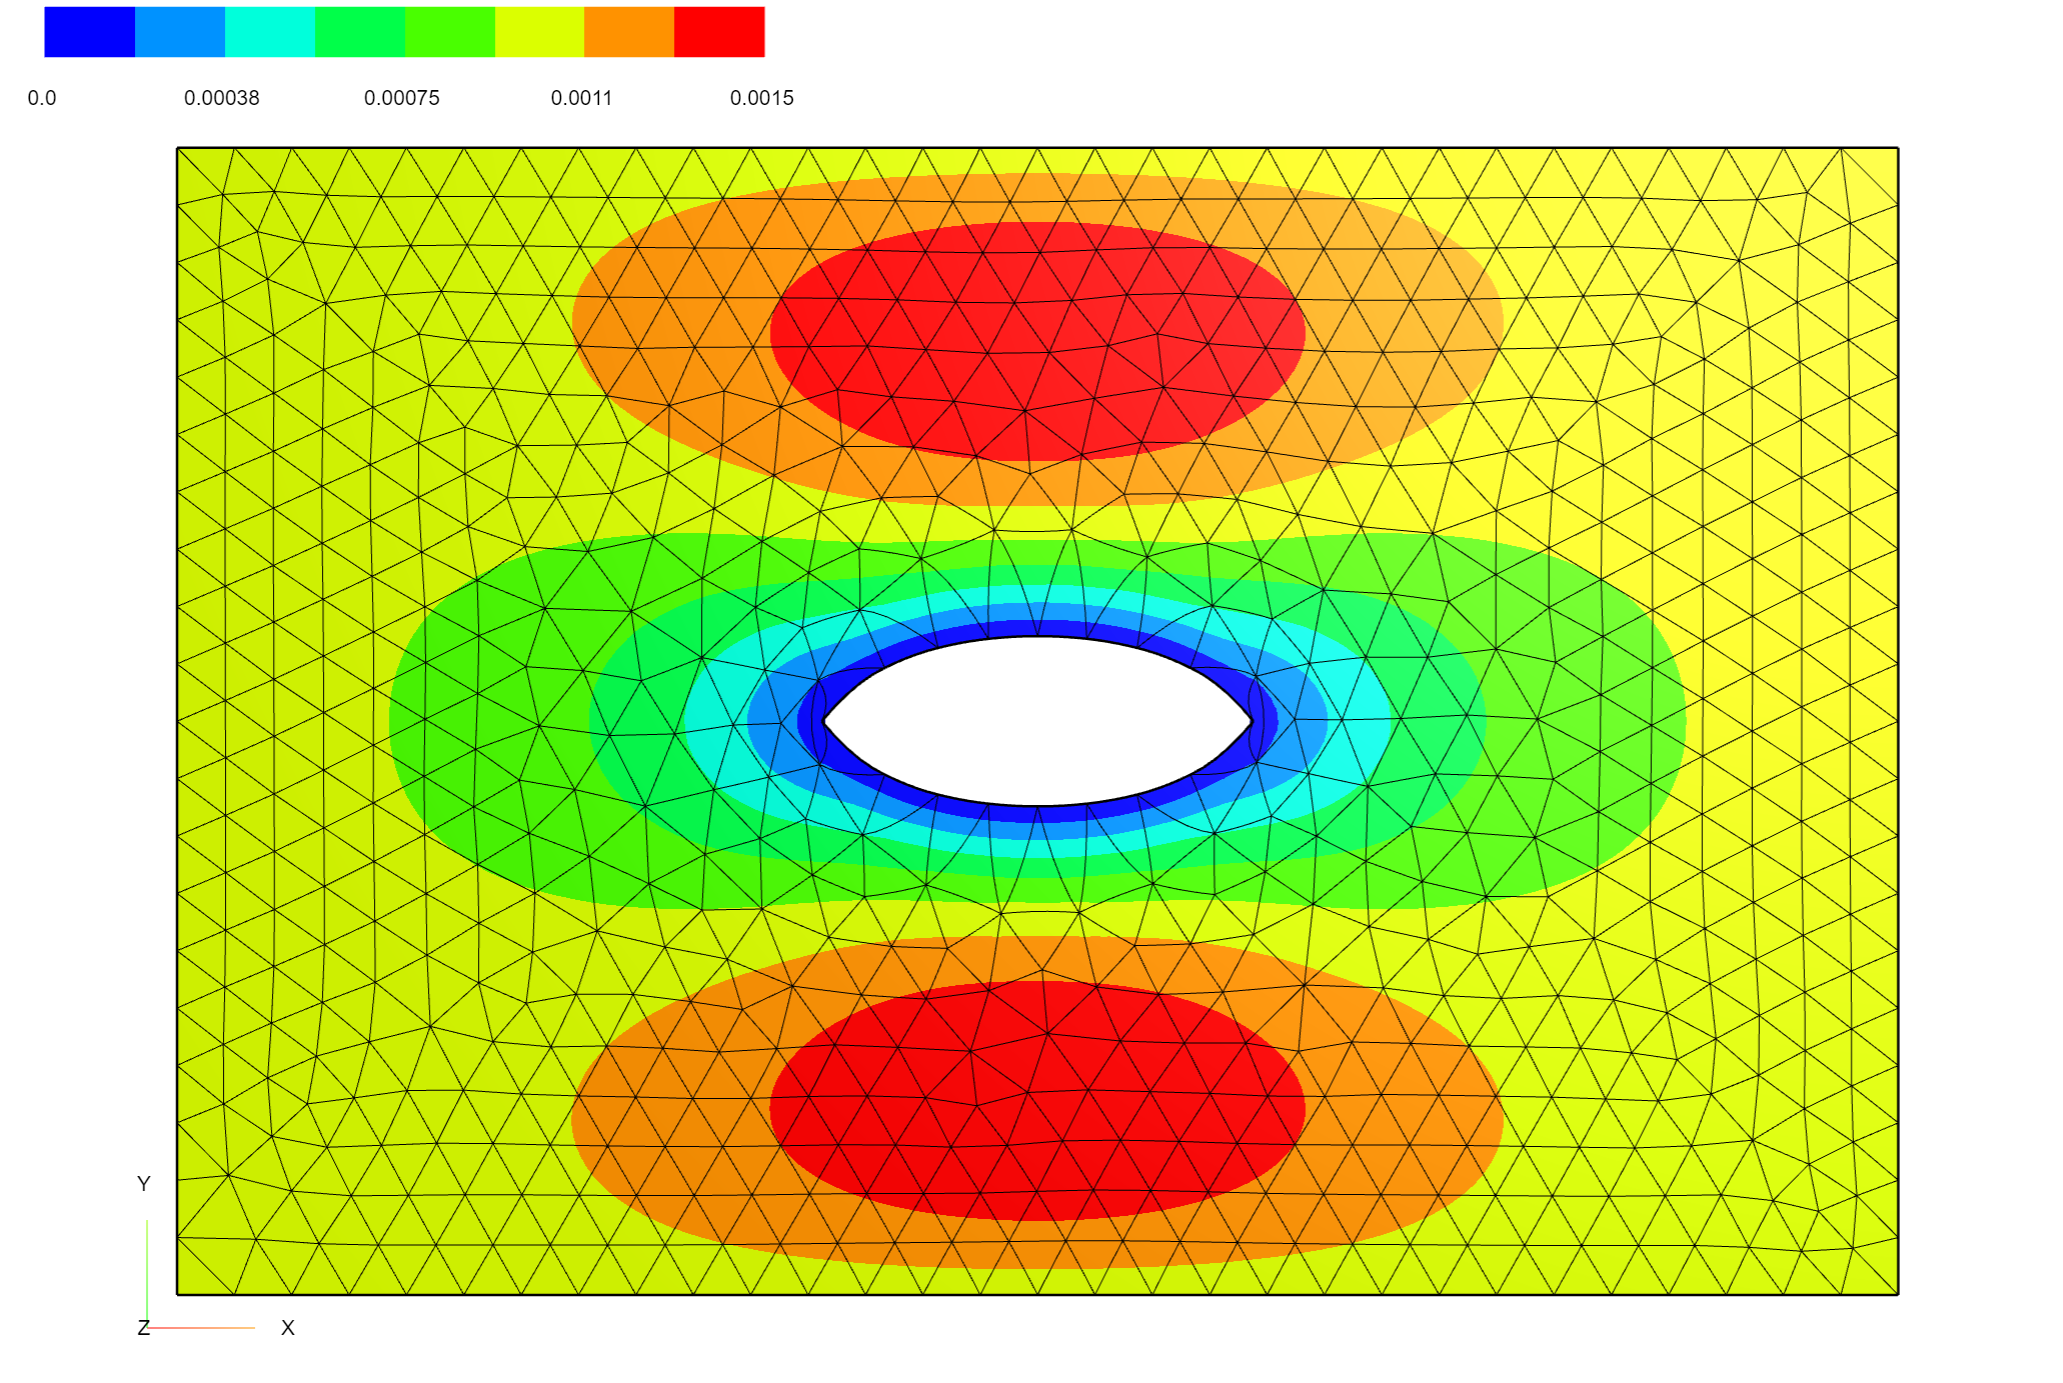
\includegraphics[width=0.8\textwidth]{figures/solution_shape_opt.PNG}
	\caption{Velocity magnitude of Stokes flow after shape optimization}
	\label{shape_opt_plot}
\end{figure}

\pagebreak

\section{The Stokes Equations in NGSolve}

The Stokes Equations are linear partial differential equations, which describe a stationary incompressible Newtonian fluid flow
with high viscosities and low Reynolds numbers. For the implementation in NGSolve, a suitable geometry and boundary conditions are 
the ones proposed by Sturm et. al. \cite{nearly_conformal_paper}, where the fluid flow around a cylinder is investigated while the
outer boundary of $\Omega$ is prescriped a velocity striclty in $x$ direction, the so called far field velocity:

\null

\begin{figure}[!htbp]
\begin{minipage}{.5\textwidth}
    \centering
    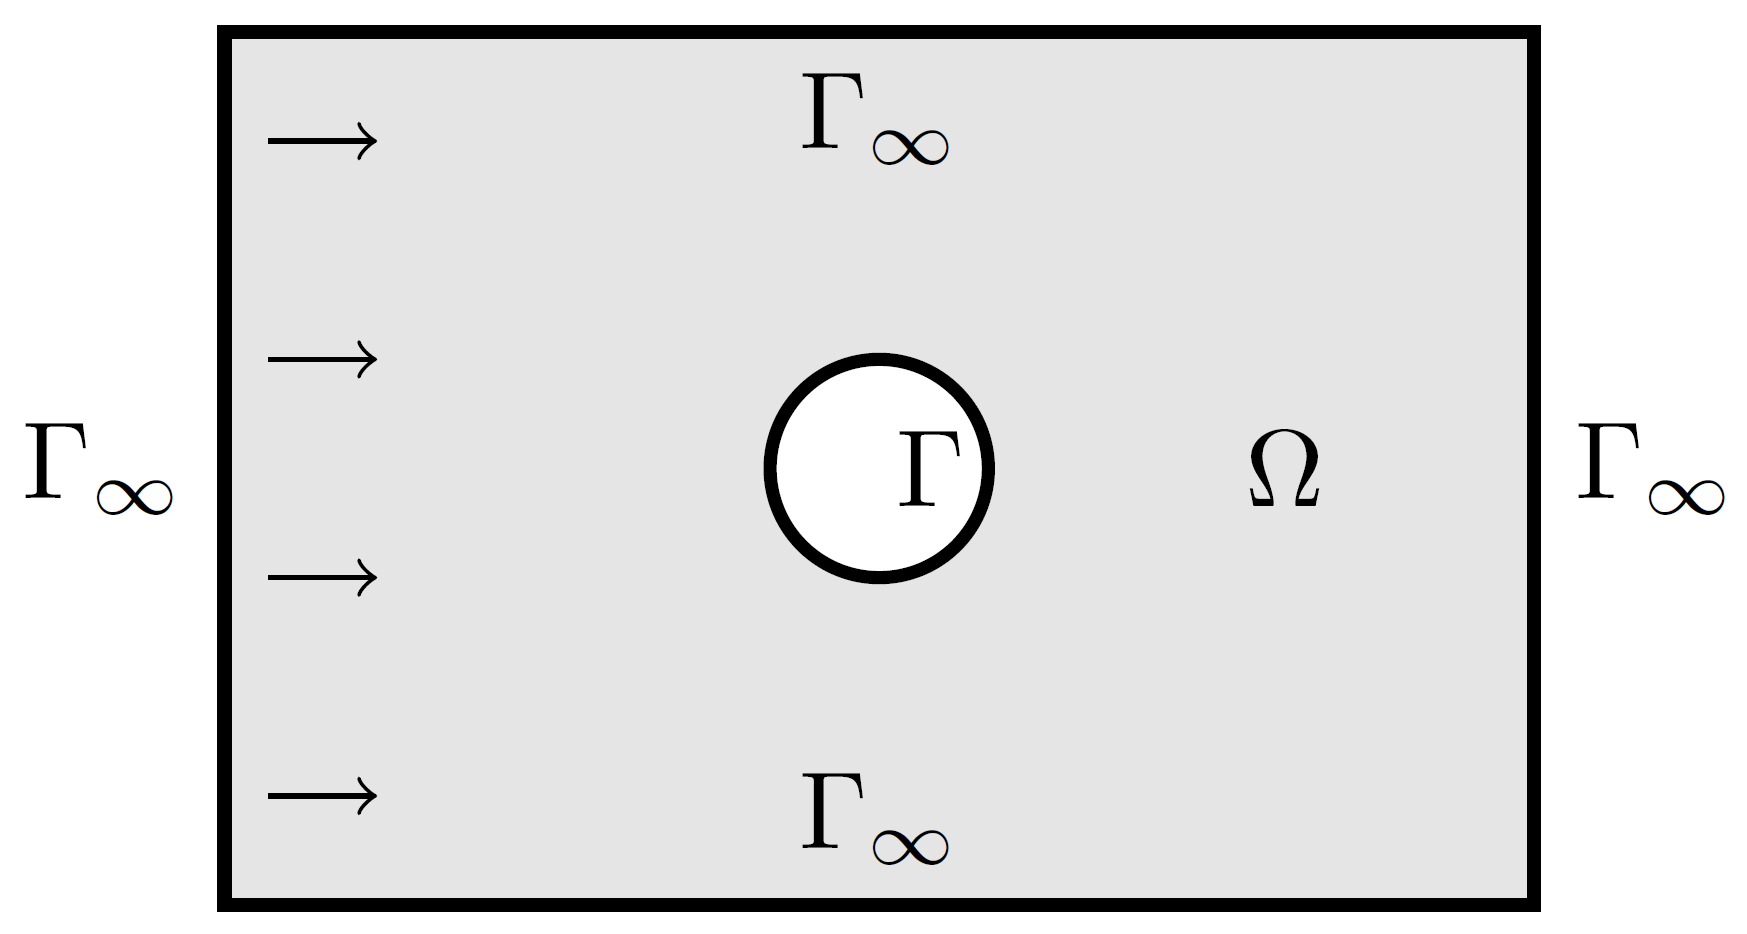
\includegraphics[width=0.8\textwidth]{figures/domain_graphic_sturm.PNG}
    \caption{Domain $\Omega$ for Stokes PDE's (\ref{stokes_PDE}) \cite{nearly_conformal_paper}}
    \label{domain_graphics}
\end{minipage}
\begin{minipage}{.5\textwidth}
    \begin{equation}\label{stokes_PDE}
        \begin{aligned}
            -\mu \Delta u + \nabla p &=0& \, &\text{in } \Omega,& \\
            \mathrm{div} \, u &=0& \, &\text{in } \Omega,& \\
            \mathbf{u} &=0& \, &\text{on } \Gamma,& \\
            \mathbf{u} &=\mathbf{u}_{\infty}& \, &\text{on } \Gamma_{\infty},& \\
        \end{aligned}
    \end{equation}
\end{minipage}
\end{figure}

\null

Where $\mu \in \mathbb{R}$ is the viscosity constant and is set to 1 for simplicity. 
The problem yields the vectorial velocity field $u:\Omega \rightarrow \mathbb{R}^d$ and 
the scalar pressure field $p:\Omega \rightarrow \mathbb{R}$. In order to solve the Stokes equation with the Finite Element Method in NGSolve,
it needs to be transformed to the weak formulation, where the solutions $u$ and $p$ are linear combinations of basis functions in a Sobolev space.
See Faustmann\cite{lecture_notes_faustmann_numPDE} Chapter 3 for further elaborations on Sobolev spaces. The weak formulation can be derrived by
multipling the now called trial-functions $u$ and $p$ with test-functions $v$ and $q$, perform transformations and integrate them. The test-functions have to fulfil certain
conditions to permit the transformations in order to arrive at a weak problem with 
linear convergence rates, see Faustmann\cite{lecture_notes_faustmann_numPDE}: \\

Find $u \in [H^1_0(\Omega)]^d$ and $p \in L^2(\Omega)$ such that
\begin{equation}\label{weak_stokes_PDE}
    \begin{aligned}
    &\int_{\Omega} \nabla \mathbf{u} : \nabla \mathbf{v} \, dx + \int_{\Omega} \mathrm{div}(\mathbf{v})p \, dx &=& \, 0 &\forall& \mathbf{v} \in [H^1_0(\Omega)]^d \\
    &\int_{\Omega} \mathrm{div}(\mathbf{u})q \, dx &=& \, 0   &\forall& q \in L^2(\Omega)
    \end{aligned}
\end{equation}

\null

Instead of considering this as a system of equations, one can look at the mixed method as one variational problem on
the product spaces $[H^1_0(\Omega)]^d \times L^2(\Omega)$, this is done by just adding both problems \cite{lecture_notes_faustmann_numPDE}:

\null

\begin{equation}\label{weak_stokes_PDE_product}
    \int_{\Omega} \nabla \mathbf{u} : \nabla \mathbf{v} \, dx + \int_{\Omega} \mathrm{div}(\mathbf{v})p \, 
    dx + \int_{\Omega} \mathrm{div}(\mathbf{u})q \, dx = \, 0 \quad \forall (\mathbf{v},q)
    \in  [H^1_0(\Omega)]^d \times L^2(\Omega)
\end{equation}

\null

In lines 19-26 of listing \ref{basic_stokes}, the variational problem \ref{weak_stokes_PDE_product} is added to
a \texttt{BilinearForm()}. After assembling of the system, in line 27-31 the non-zero Dirichlet conditions are assigned. 
When setting up the geometry, the boundaries already have to be named to do the boundary conditions assignment. The geometry
shown in figure \ref{domain_graphics}, is defined in the beginning in lines 5-11.


\pagebreak

\begin{lstlisting}[language=Python, title=Basic Stokes PDE's with Python3 and NGSolve, label=basic_stokes]
    k = 2
    V = H1(mesh,order=k, dirichlet="top|bot|cyl|in|out")
    Q = H1(mesh,order=k-1)
    FES = FESpace([V,V,Q])
    ux,uy,p = FES.TrialFunction()
    vx,vy,q = FES.TestFunction()
    def Equation(ux,uy,p,vx,vy,q):
        div_u = grad(ux)[0]+grad(uy)[1] # custom divergence u
        div_v = grad(vx)[0]+grad(vy)[1] # custom divergence v
        return (grad(ux)*grad(vx)+grad(uy)*grad(vy) + div_u*q + div_v*p)* dx
    a = BilinearForm(FES)
    a += Equation(ux,uy,p,vx,vy,q)
    a.Assemble()
    gfu = GridFunction(FES)
    uinf = 0.001
    uinf_c = CoefficientFunction((uinf))
    gfu.components[0].Set(uinf_c, definedon=mesh.Boundaries("in|top|bot|out"))
    def solveStokes():
    res = gfu.vec.CreateVector()
    res.data = -a.mat * gfu.vec
    inv = a.mat.Inverse(FES.FreeDofs())
    gfu.vec.data += inv * res
    scene_state.Redraw()
\end{lstlisting}

Below the solution obtained with NGSolve (see listing \ref{basic_stokes}). On the surface of the cylinder, 
the no-slip condition (standard Dirichlet = 0) can be observed. Also an intuitive observation of the fulfilled continuity can be made:
where the cross section is smaller, e.g. in $x$ vicinity of the cylinder, the velocity is increased:

\begin{figure}[ht]
    \centering
    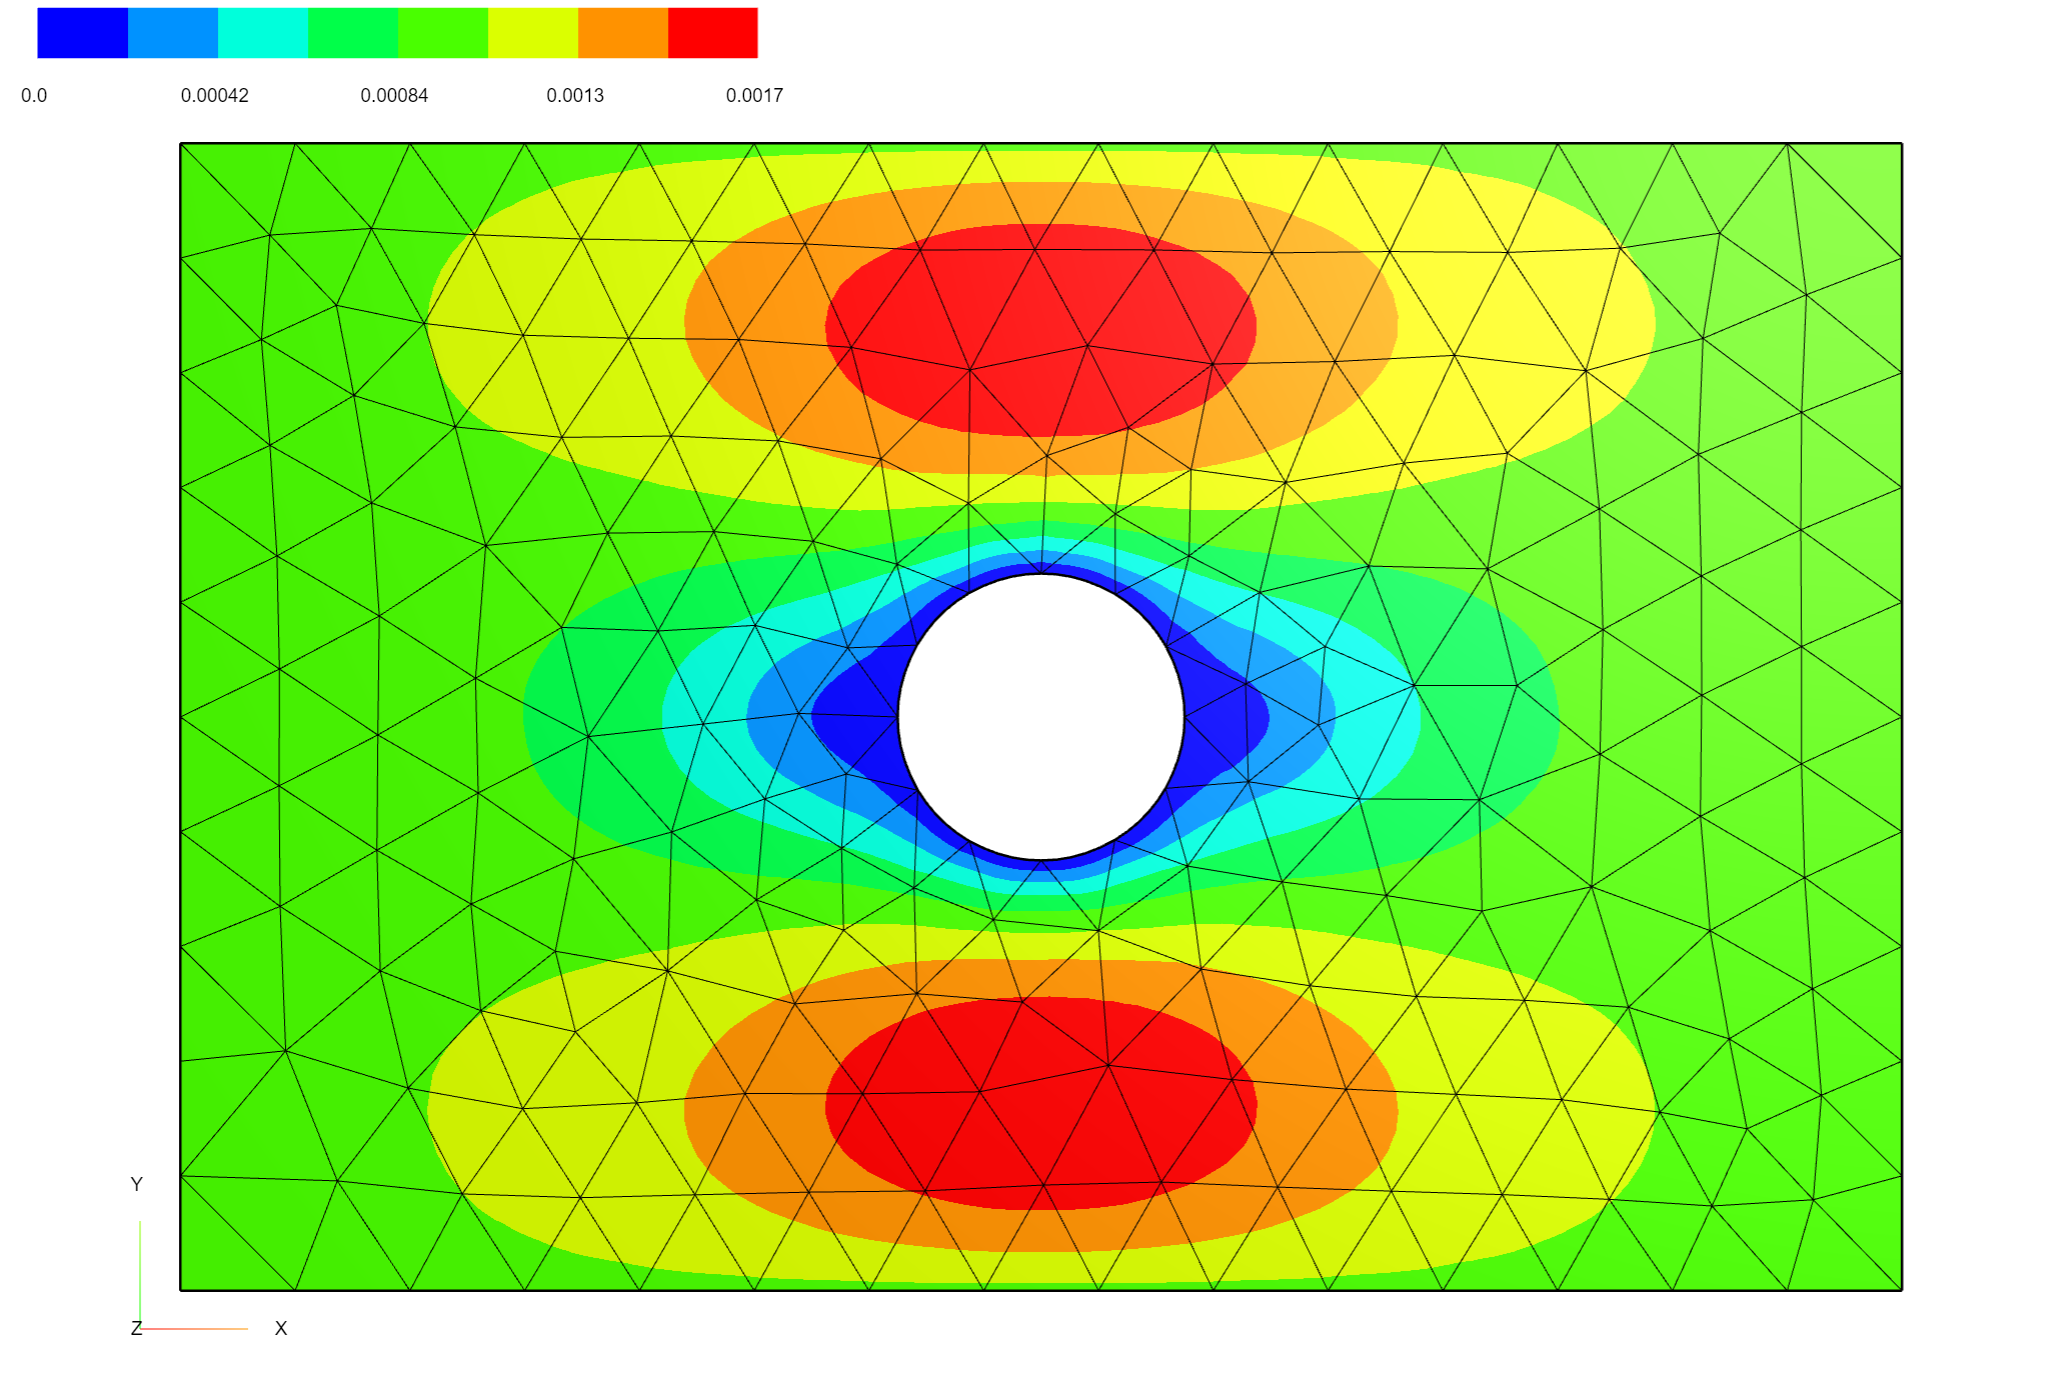
\includegraphics[width=0.92\textwidth]{figures/solution_stokes_basic.PNG}
	\caption{Surface Plot - Velocity $||\mathbf{u}||_2$ of Stokes Flow - FEM solution to problem (\ref{stokes_PDE})}
	\label{basic_stokes_flow_plot}
\end{figure}

\pagebreak

\section{Differentiability}

\vfill

As explained in the introduction, the existence of the shape derivative needs to be shown.
The perturbations of the shape $\Omega$ are described by the following transformation: $\Omega_t := (Id + tX )(\Omega)$ where.
For small perturbations and $t > 0$, the shape derivative is: \cite{fully_semi_paper_sturm}

\begin{equation}\label{shape_derrivative_t_limit}
	DJ(\Omega)(X) := \left(\frac{\partial}{\partial t}J(\Omega_t)\right)\bigg\rvert_{t=0} = \lim_{t \to 0} \frac{J(\Omega_t)-J(\Omega)}{t}
\end{equation}
This notion of the shape derivative is used in this chapter in the context of differentiability. The functional that returns a scalar quantity 
represetative of the energy dissipation is shown here where : is the Frobenius product and $\mathrm{D} \mathbf{u}$ is the Jacobi matrix of $\mathbf{u}$.
\begin{align}\label{energy_dissipation_equation}
	J(\Omega) = \frac{1}{2} \int_{\Omega} \mathrm{D} \mathbf{u} : \mathrm{D} \mathbf{u} \, \mathrm{dx}
\end{align}
Sturm et. al. \cite{nearly_conformal_paper} proposed the shape derrivative of following form is given by: \\
Shape Derivative of $J$ at $\Omega$ in direction $ X \in [C^{0,1}(\bar{\Omega})]^2 $
\begin{align}\label{shape_derivative_S1}
	\mathrm{d}J(\Omega)(X) &= \int_{\Omega} \mathrm{S}_1 : \mathrm{D}X \, \mathrm{dx} \\
	\mathrm{S}_1 &= \left( \frac{1}{2}\mathrm{D} \mathbf{u} : \mathrm{D} \mathbf{u} - p \, \mathrm{div}(\mathbf{u}) \right)
	\mathrm{I}_2 + \mathrm{D} \mathbf{u}^{\top}p - \mathrm{D} \mathbf{u}^{\top} \mathrm{D} \mathbf{u}
\end{align}
where $(\mathbf{u},p)$ solve (\ref*{weak_stokes_PDE_product})
\begin{theorem}
let $X \in [C^{0,1}(\bar{\Omega})]^2$ with $X = 0$ on $\Gamma_{\infty}$ be a given vectorfield. \\
Set $\mathrm{T}_t(.) := \mathrm{id} + tX $ , with $t \in \mathbb{R}$ and $\Omega_t := \mathrm{T}_t(\Omega)$, where 
$(\mathbf{u}_t, p_t)$ solve (\ref{weak_stokes_PDE_product}) and $\Omega$ is replaced by $\Omega_t$ s.t. \\
$p_t \in \mathrm{L}^2(\Omega_t), \int_{\Omega_t} p_t \, \mathrm{dx} = 0 $ and $\mathrm{u}_t \in [H^1(\Omega_t)]^2:$ 
\begin{align}
	\int_{\Omega_t} \mathrm{D} \mathbf{u}_t : \mathrm{D} \mathbf{\mathbf{v}} + \mathrm{div}(\mathbf{v}) \, p_t + \mathrm{div}(\mathbf{u}_t) \, q \, dx = \, 0 \quad \forall (v,q)
    \in  [H^1_0(\Omega_t)]^d \times L^2(\Omega_t)
\end{align}
Introduction of change of variables shows that $(\mathbf{u}^t, p^t) := (\mathbf{u}_t \circ \mathrm{T}_t, p_t \circ \mathrm{T}_t)$ satisfy:
\begin{equation}
\begin{aligned}\label{trafo_weak_stokes}
	&\int_\Omega \mathrm{det}(\mathrm{DT}_t)
	\left( \mathrm{DT}_t^{-1} \mathrm{D}\mathbf{u}^t:\mathrm{DT}_t^{-1} \mathrm{D}\mathbf{v} -p\, \mathrm{tr}(\mathrm{D}\mathbf{v}\mathrm{DT}_t^{-1})  +
	q \, \mathrm{tr}(\mathrm{D}\mathbf{u}\mathrm{DT}_t^{-1}) \right) \mathrm{dx} \\
	& \quad \quad \quad \quad \quad \quad \quad \quad \quad \ \forall (v,q) \in [H^1(\Omega)]^2 \times L^2(\Omega)
\end{aligned}
\end{equation}
with:
\begin{align*}
	\mathrm{D}\mathbf{v}\circ\mathrm{T}_t &= \mathrm{D}(\mathbf{v}\circ\mathrm{T}_t) \\
	\mathrm{div}(\mathbf{v}) &= \mathrm{tr} \left( \mathrm{D}(\mathbf{v} \circ \mathrm{T}_t)(\mathrm{DT}_t^{-1}) \right)
\end{align*}

\vfill

\pagebreak

The functional $J(\Omega,\mathbf{u})$ is now reduced to the functional $J(\Omega)$, since the change of the quantities $(\mathbf{u},p)$
is taken into account by the transformation theorem. The minimum of (\ref{energy_dissipation_equation})
satisfies the saddlepoint problem (\ref{trafo_weak_stokes}). It can be obtained with the Lagrange Multiplier method, 
see Faustmann \cite{lecture_notes_faustmann_numPDE}. The corresponding Lagrangian which can be used to minimize (\ref{energy_dissipation_equation})
is:
\begin{equation}
 \begin{aligned}
	\mathcal{L}(t,\mathbf{v}, q) = \frac{1}{2}& \int_{\Omega} \mathrm{det}(\mathrm{DT}_t) \mathrm{D} \mathbf{v}(\mathrm{DT}_t)^{-1} :
	\mathrm{D} \mathbf{v}(\mathrm{DT}_t)^{-1} \, \mathrm{dx} \\
	&- \int_{\Omega}\mathrm{det}(\mathrm{DT}_t)q \, \mathrm{tr} \left( \mathrm{D}\mathbf{v}(\mathrm{DT}_t)^{-1} \right)
\end{aligned}
\end{equation}
To find the shape derivative, one can now derive this parametrized Lagrangian, for details on the derivation of parametrized Lagrangians, 
see K. Ito et. al. \cite{lagrangian_derivative}. With the derivative of the Lagrangian obtained, it holds true that:
\begin{align}
	\mathrm{d}J(\Omega)(X) =\ \frac{\mathrm{d}}{\mathrm{d}t} \mathcal{L}(t, \mathbf{u}^t, 0)\big\rvert_{t=0}  =
	\frac{\partial}{\partial t}\mathcal{L}(0,\mathbf{u},p) = \int_{\Omega} \mathrm{S}_1 : \mathrm{D}X \, \mathrm{dx} 
\end{align}
\qed
\end{theorem}



\pagebreak

\section{Augmented Lagrangian and Geometric Constraints}

In the previous chapter, the differentiability of the shape function with respect to the perturbation 
parameter $t$ was recapitulated \cite{nearly_conformal_paper}. One can now employ a minimization problem
which yields an approximative solution. This is where the Augmented Lagrangian is introduced. Since differentiability was shown,
one can show that the negative derrivative of the Augmented Lagrangian is an approximate minimizer to the 
Lagrangian (\ref{parametrized_lagrangian}), for elaborations on Augmented Lagrangians see Sturm Lecture Notes \cite{lecture_notes_sturm}. 
One considers again the Lagrangian (\ref{parametrized_lagrangian}) in the unparametrized way which can be evaluated on the FEM mesh:
\begin{equation}\label{basic_lagrangian}
	%L(\Omega,u,p) = 
    \mathcal{L}(\Omega) = \frac{1}{2} \int_{\Omega} \mathrm{D}\mathbf{u}: \mathrm{D} \mathbf{u} \, \mathrm{dx} + 
	\int_{\Omega} \nabla \mathbf{u} : \nabla \mathbf{u} \, \mathrm{dx} + \int_{\Omega} \mathrm{div}(\mathbf{u})p \, \mathrm{dx} +
	 \int_{\Omega} \mathrm{div}(\mathbf{u})p \, \mathrm{dx}
\end{equation}
If one minimizes this problem, one can observe: the numerical scheme will just make the obstacle smaller since this will 
result in a minimization of the drag as well. This is not a trivial result but also not a result of interest. Therefore one analyzes the 
volume and barycenter of the obstacle and formulates terms that penalize deviations from the initial values of the volume and barycenter.
\begin{align}
    \mathrm{vol}(\Omega) &= \int_{\Omega} 1 \ \mathrm{dx} \in \mathbb{R} \label{vol_equation}\\
    \mathcal{L}^2_{\mathrm{vol}}(\Omega) &= \alpha \ \Big( \mathrm{vol}( \mathbf{T}_{t}(\Omega) )-\mathrm{vol}(\Omega_0) \Big) ^2
\end{align}
The quantity $\mathcal{L}_{\mathrm{vol}}(\Omega)$ is a quadratically penalized term that is easy to derrive and is used to formulate 
the Augmented Lagrangian. If the deformed domain $\Omega$ yields an obstacle of identical volume, the term is zero, deviations 
from the initial obstacle volume are penalized. The same is done for the barycenter of the obstacle. 
\begin{align}
    \mathrm{bc}(\Omega) =
    \frac{1}{\mathrm{vol}(\Omega)}\int_{\Omega} \mathbf{x} \ \mathrm{d} \mathbf{x} \in \mathbb{R}^2
\end{align}
Since it is a vectorial quantity, the integral is decomposed into its components such that it yields a scalar quantity:
\begin{align}
    \mathrm{bc}_x(\Omega) &=
    \frac{1}{\mathrm{vol}(\Omega)}\int_{\Omega} x \ \mathrm{dx} \, , \quad 
    \mathrm{bc}_y(\Omega) =
    \frac{1}{\mathrm{vol}(\Omega)}\int_{\Omega} y \ \mathrm{dx} \label{bc_equation}\\
	\mathcal{L}^2_{\mathrm{bc}}(\Omega) &= \beta \Big( \mathrm{bc}_x( \mathbf{T}_{t}(\Omega) )-\mathrm{bc}_x(\Omega_0) \Big)^2 + 
	\gamma\Big( \mathrm{bc}_y( \mathbf{T}_{t}(\Omega) )-\mathrm{bc}_y(\Omega_0) \Big)^2
\end{align}
Finally, the quadratically penalized Augmented Lagrangian:
\begin{align}\label{final_aug_lagrange}
	\mathcal{L}_{\mathrm{aug}}(\Omega) =  \mathcal{L}(\Omega) + \mathcal{L}^2_{\mathrm{vol}}(\Omega) + \mathcal{L}^2_{\mathrm{bc}}(\Omega)
\end{align}
The parameters $\alpha$, $\beta$ and $\gamma$ are used to weigh the quadratically penalized terms and vary them dynamically while
iterating. \\

Remark: The quadratically penalized terms do not evaluate the surface and barycenter of the obstacle and its deviations, but rather
of the entire domain $\Omega$, but since the obstacle is in the center and the entire geometry symmetric, the obtained quantities are representative of
the surface and barycenter of the obstacle as well.





\pagebreak


\section{Shape Derivative in NGSolve}\label{shape_der_chapter}
\subsection{Derivative of the Augmented Lagrangian}

After the Augmented Lagrangian is set up accordingly, the derivatives $\mathrm{d}\mathcal{L}_{\mathrm{i}}(\Omega)(X)$ can be formulated and implemented.
In the NGSolve implementation, analytical derivatives for the terms $\mathrm{d}\mathcal{L}^2_{\mathrm{bc}}(\Omega)(X)$ 
and $\mathrm{d}\mathcal{L}^2_{\mathrm{vol}}(\Omega)(X)$ are directly used. The definition for $\mathrm{vol}(\Omega)$ is equal to
the definition in equation (\ref{vol_equation}) and $\mathrm{bc}_{x,y}(\Omega)$ are equal to the definitions in equation (\ref{bc_equation}).\\

The derivative of the volume constraint term in $X$ direction is given by
\begin{equation}\label{eq:constraints_vol}
	%L(\Omega,u,p) += 
	\mathrm{d}\mathcal{L}^2_{\mathrm{vol}}(\Omega)(X) = 2 \, \alpha \Big( (\mathrm{vol}(\Omega) - \mathrm{vol}(\Omega_0) \Big) \, \mathrm{div}(X)
\end{equation}
And the derivative of the barycenter constraint term in $X$ direction is given by
\begin{equation}\label{eq:constraints_bc}
	\begin{aligned}
	\mathrm{d}\mathcal{L}^2_{\mathrm{bc}}(\Omega)(X) =
	2& \, \beta \Big( \mathrm{bc}_x(\Omega) - \mathrm{bc}_x(\Omega_0) \Big) \, \int_{\Omega} \frac{1}{\mathrm{vol}(\Omega)^2} \, \mathrm{div}(X) \, x 
	+ \frac{1}{\mathrm{vol}(\Omega)} \, \mathrm{div}(X) \, x \cdot \vec{e}_x \, X \, \mathrm{dx} \\
	+& \, 2 \, \gamma \Big( \mathrm{bc}_y(\Omega) - \mathrm{bc}_y(\Omega_0) \Big) \, \int_{\Omega} \frac{1}{\mathrm{vol}(\Omega)^2} \, \mathrm{div}(X) \, y 
	+ \frac{1}{\mathrm{vol}(\Omega)} \, \mathrm{div}(X) \, y \cdot \vec{e}_y \, X\, \mathrm{dx}.
	\end{aligned}
\end{equation}
\\
To obtain the term $\mathrm{d}\mathcal{L}(\Omega)(X)$, the NGSolve command \fun{DiffShape(X)} is used, to utilize the library's Automatic Differentiation
capabilites. Finally one arrives at the shape derivative that is, to reiterate, the derivative of the Augmented Lagrangian

\begin{align}
	\mathrm{d}\mathcal{L}_{\mathrm{aug}}(\Omega)(X) = \mathrm{d}\mathcal{L}(\Omega)(X) + \mathrm{d}\mathcal{L}^2_{\mathrm{vol}}(\Omega)(X) 
	+ \mathrm{d}\mathcal{L}^2_{\mathrm{bc}}(\Omega)(X).
\end{align}
In listing \ref{lagrangian_derivative_code} the implementation in NGSolve, for more details see either appendix \ref{final_code} or the 
\fun{JupyterNotebook}
\begin{lstlisting}[language=Python, title=Derivative of Augmented Lagrangian, label=lagrangian_derivative_code]
	# Initilize LinearForm object
	dLOmega = LinearForm(VEC)
	# add automatic shape differentiation term to LinearForm object
	dJOmega += Lagrangian.DiffShape(X)
	# add analytically derived volume constraint term to LinearForm object
	vol = Parameter(1)
	vol.Set(Integrate(surf_t,mesh))
	alpha0 = 1e-4
	alpha = Parameter(alpha0)
	dLOmega += 2*alpha*(vol-surf_0)*div(X)*dx
	# add analytically derived x-barycenter constraint term to LinearForm object
	beta0 = 1e-3
	beta = Parameter(beta0)
	bc_x = Parameter(1)
	bc_x.Set((1/surf_0)*Integrate(bc_tx,mesh))
	dJOmega += 2*beta*(bc_x-bc_0x)*((1/vol**2)*div(X)*x+(1/vol)*div(X)*x*sum(gfset.vecs[0].data)[0])*dx
	# add analytically derived y-barycenter constraint term to LinearForm object
	bc_y = Parameter(1)
	bc_y.Set((1/surf_0)*Integrate(bc_ty,mesh))
	dJOmega += 2*beta*(bc_y-bc_0y)*((1/vol**2)*div(X)*y+(1/vol)*div(X)*y*sum(gfset.vecs[0].data)[1])*dx
\end{lstlisting}


\pagebreak

\subsection{Deformation}
The deformation, as described in the mathematical sense is the $X$ in $\Omega_t := (Id + tX )(\Omega)$.
Its according space is \obj{H1(mesh, order=2, dim=2)}, with dirichlet boundaries on the outsides of the square.

This variable in our ngsolve implementation is called \var{gfX}. This is a two-dimensional \obj{GridFunction} which is computed from the shape derivative and stores the information how to deform the mesh at each node.

The shape derivative is the linear form \var{dJOmega} in our code. Since the goal is, to make steps in a descent direction (negative), we have to make sure we only calculate according solutions.
This is done by setting the bilinear form of this problem to the $H^1$ norm.

\begin{equation}
	\partial J(\Omega) = \int(\phi\cdot X)+(\nabla\phi\cdot \nabla X) \, dx
\end{equation}

This always yields a positive value, if we subtract instead of add this value, we minimize the shape function.

% is this even useful?
\begin{lstlisting}[language=Python, title=Solving For The Deformation, label=lst:deformation_solve]
def SolveDeformationEquation():
	rhs = gfX.vec.CreateVector()
	rhs.data = dJOmega.vec - b.mat * gfX.vec
	update = gfX.vec.CreateVector()
	update.data = b.mat.Inverse(VEC.FreeDofs()) * rhs
	gfX.vec.data += update
\end{lstlisting}

Since the minimization is done in iterations, we have to keep track of the previous deformations. This is done in ngsolve by adding the parts of \var{gfX} to another variable called \var{gfset}. This \var{gfset} is then always used to call \fun{SetDeformation()} on the mesh.
With each call, this adds the \var{gfset} onto the mesh. To circumvent this, after each iteration \fun{UnsetDeformation()} is called.

To not overshoot anything, instead of adding the entire \var{gfX} to \var{gfset}, it is scaled by a number divided by its norm. That way we can make sure, that each iteration deforms the mesh in small, similar sized steps.
There is still one inconsistency: the \var{gfX} can also deform nodes inside the mesh, which change nothing for the real solution, but count towards this norm. That problem is solvable, by integrating this \obj{GridFunction} over its boundary. Since the outside of our square are dirichlet boundaries, this way only the changes on the obstacle are measured.






\pagebreak

\section{Iteration}

Since the minimization is done in iterations, we have to keep track of the previous 
deformations. This is done in ngsolve by adding the parts of \var{gfX} to another 
variable called \var{gfset}. This \var{gfset} is then always used to call \fun{SetDeformation()}
 on the mesh. With each call, this adds the \var{gfset} onto the mesh. To circumvent this, 
 after each iteration \fun{UnsetDeformation()} is called. To not overshoot anything, 
 instead of adding the entire \var{gfX} to \var{gfset}, it is scaled by a number divided 
 by its norm. That way we can make sure, that each iteration deforms the mesh in small, 
 similar sized steps. There is still one inconsistency: the \var{gfX} can also deform 
 nodes inside the mesh, which change nothing for the real solution, but count towards this 
 norm. That problem is solvable, by integrating this \obj{GridFunction} over its boundary. 
 Since the outside of our square are dirichlet boundaries, this way only the changes on the 
 obstacle are measured. Another important thing to be aware of is, that symmetric deformations
  around an obstacle might cancel each other out in the integral. This is circumvented by 
  calculating with the squared values.

In this chapter we want do describe the process of one iterations which gets repeated time after time until the optimal shape is achieved.

There are a few parameters that are recalculated or conditionally updated through the iterations. This includes the current volume and barycenter values, their respective scalings $\alpha$ and $\beta$, and $gamma$ for the Cauchy Riemann terms that ensure a better mesh quality.

Before we start with the iteration process we reset all possible variables:
This includes the \var{gfset}, resetting the scene, and to reinitialize the parameters for the geometric constraints. If this step is skipped, one could start with weird variable values that lead to drastically different results.

\begin{lstlisting}[language=Python, title=Reset before iteration, label=lst:reset]
gfset.Set((0,0))
mesh.SetDeformation(gfset)
scene.Redraw()
updateParams()
alpha0 = 1e-4
beta0 = 1e-0
gamma0 = 1e2
alpha.Set(alpha0)
beta.Set(beta0)
gamma.Set(gamma0)
iter_max = 750
\end{lstlisting}

This iteration is bounded by a maximum number of steps, even though it is also be possible to take some measure on the \var{gfX} and determine a stop by it.
This still requires parameter tuning, especially because some measures could yield different results depending on the mesh width.
Other possibilities for breaks in the loop are a maximum number for the scaling parameters e.g. $\alpha$ or a very small difference in the drag from one iteration to the next.

Each iteration then starts by calling \fun{SetDeformation(gfset)}, and redrawing needed scenes. This would also be the place to gather data, like the current drag or area of the mesh, etc.

Afterwards we start calculating towards the next step:
We Assemble the state equation bilinear form and solve it over this newly deformed mesh. Following this we assemble the linear and bilinear form for the shape derivative and solve for a new deformation. After this is done, one can already use \fun{UnsetDeformation()} and the last thing to do is updating values.

We scale the \var{gfX} to its desired magnitude and subtract it from \var{gfset}. At this point it is also wise to check for some measure of close we are to a good solution and for example increase the parameters for the geometric constraints.

The entire code inside the loop looks like this:

\begin{lstlisting}[language=Python, title=Iteration, label=lst:loop]
		mesh.SetDeformation(gfset)
		scene.Redraw()
		data.append(vol.Get())
		a.Assemble()
		solveStokes()
		b.Assemble()
		dLOmega.Assemble()
		SolveDeformationEquation()
		updateParams()
		mesh.UnsetDeformation()
		gfxnorm = Norm(gfX.vec)
		scale = 0.01 / gfxnorm
		
		if(gfxnorm < 1e-5):
			if alpha.Get() < 1:
				increaseParams(2,True)
			else:
				break
		gfset.vec.data -= scale * gfX.vec
\end{lstlisting}

It is also possible to implement some sort of line search for the step size, similar to the armijo rule. This way one can do less iterations but take better/bigger steps, being more efficient in regards to computational efforts. More to this can be read in ...

\pagebreak

\section{Results and Conclusion}
\subsection{General Results and Agreement with Literature}
\begin{figure}[h]
\begin{minipage}{.5\textwidth}
    \centering
    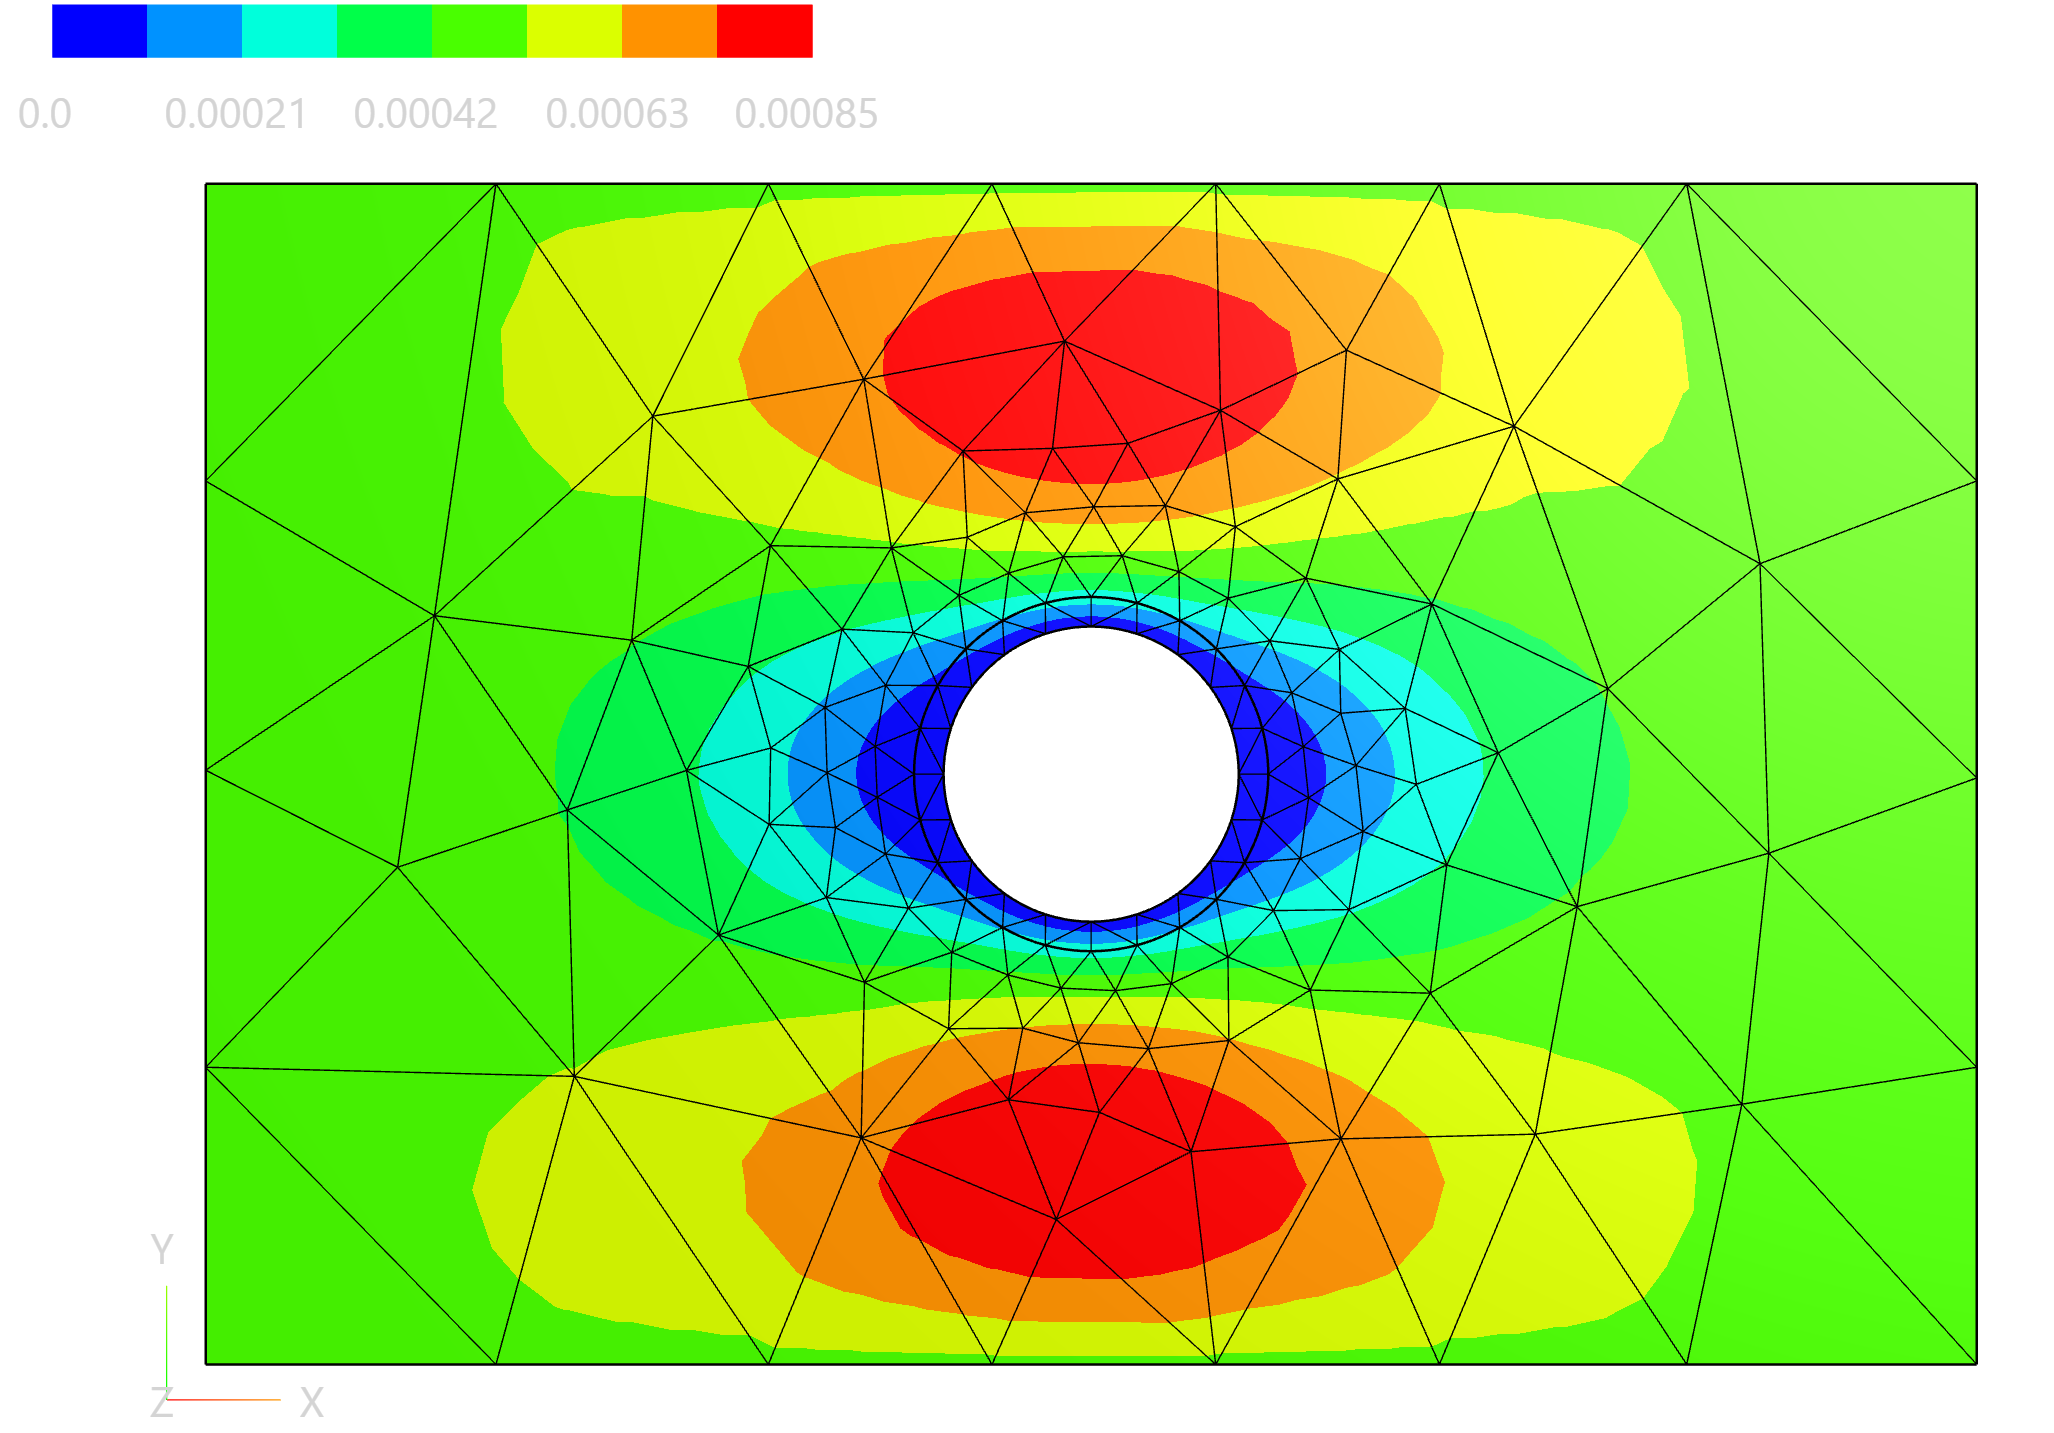
\includegraphics[width=1\textwidth]{figures/u_0.PNG}
    \caption{ $\mathbf{||u||_2}$ on $\Omega_{\mathrm{n}}$ for $\mathrm{n}=0$}
    \label{plot_ref_u_0}
\end{minipage}
\begin{minipage}{.5\textwidth}
    \centering
    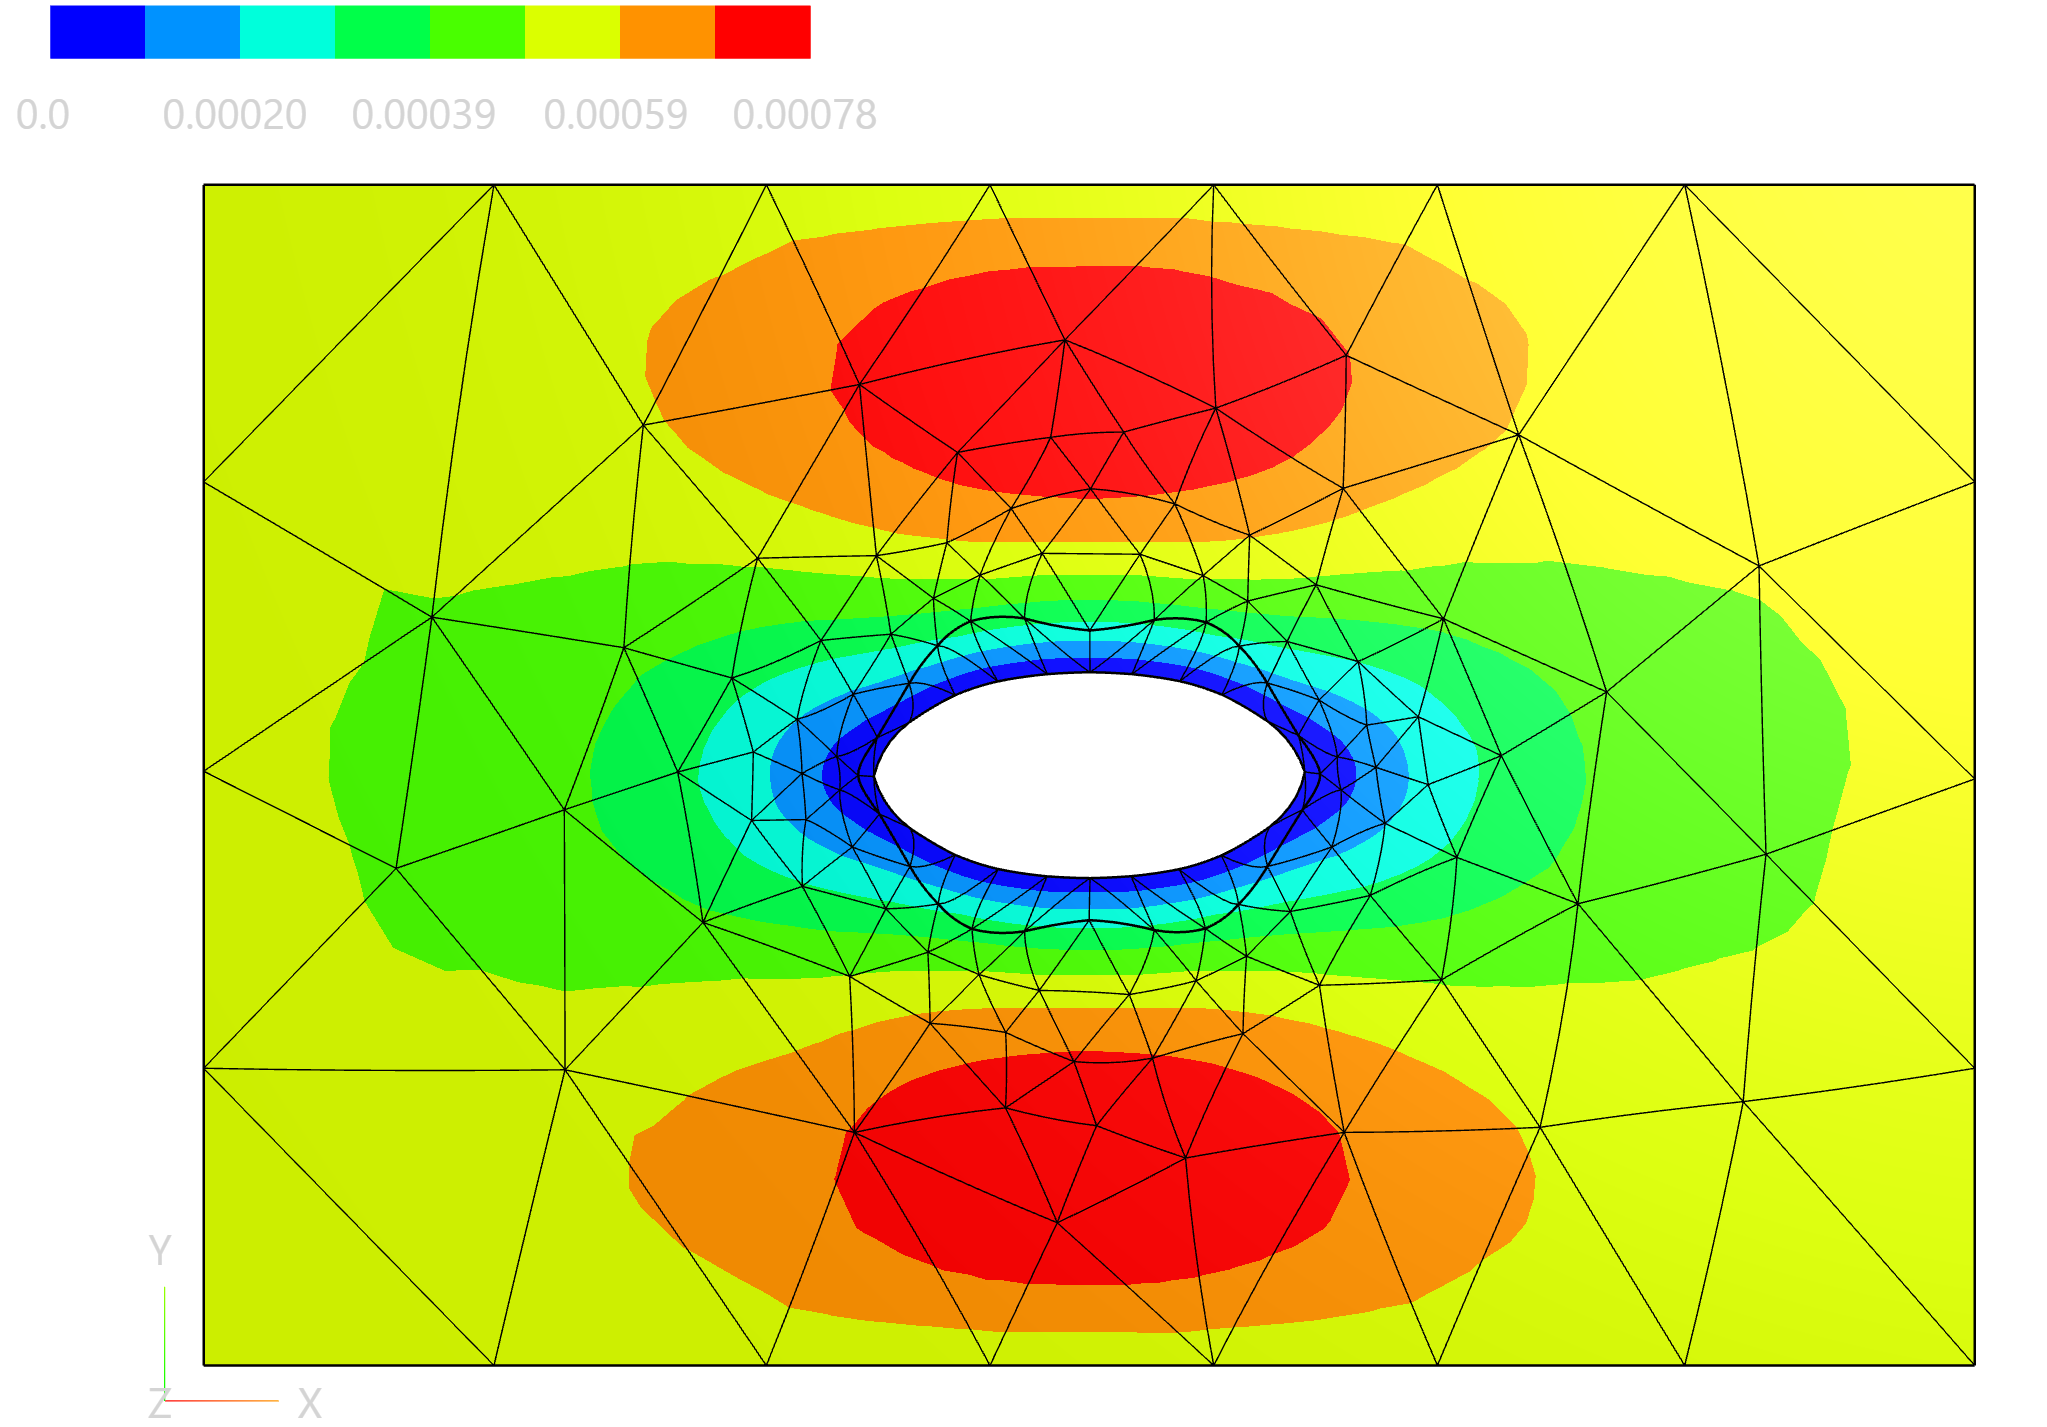
\includegraphics[width=1\textwidth]{figures/u_final.PNG}
    \caption{ $\mathbf{||u||_2}$ on $\Omega_{\mathrm{n}}$ for $\mathrm{n}=800$}
    \label{plot_ref_u_final}
\end{minipage}
\end{figure}

In the figures \ref{plot_ref_u_0} and \ref{plot_ref_u_final} above, the initial and final domains $\Omega$ 
show good agreement with the results obtained by Sturm et. al. \cite{fully_semi_paper_sturm} where the 
tips of the ogive show approximately 45 degree angles. The constraint for near conformality posed in equation
(\ref{eq_conf_aux}) also yields acceptable mesh quality at the tips, where the mesh withouth these contraints
would result in a self intersecting mesh. This renders the Stokes solution $(\mathbf{u},p)$ useless locally.

\begin{figure}[h]
    \begin{center}
        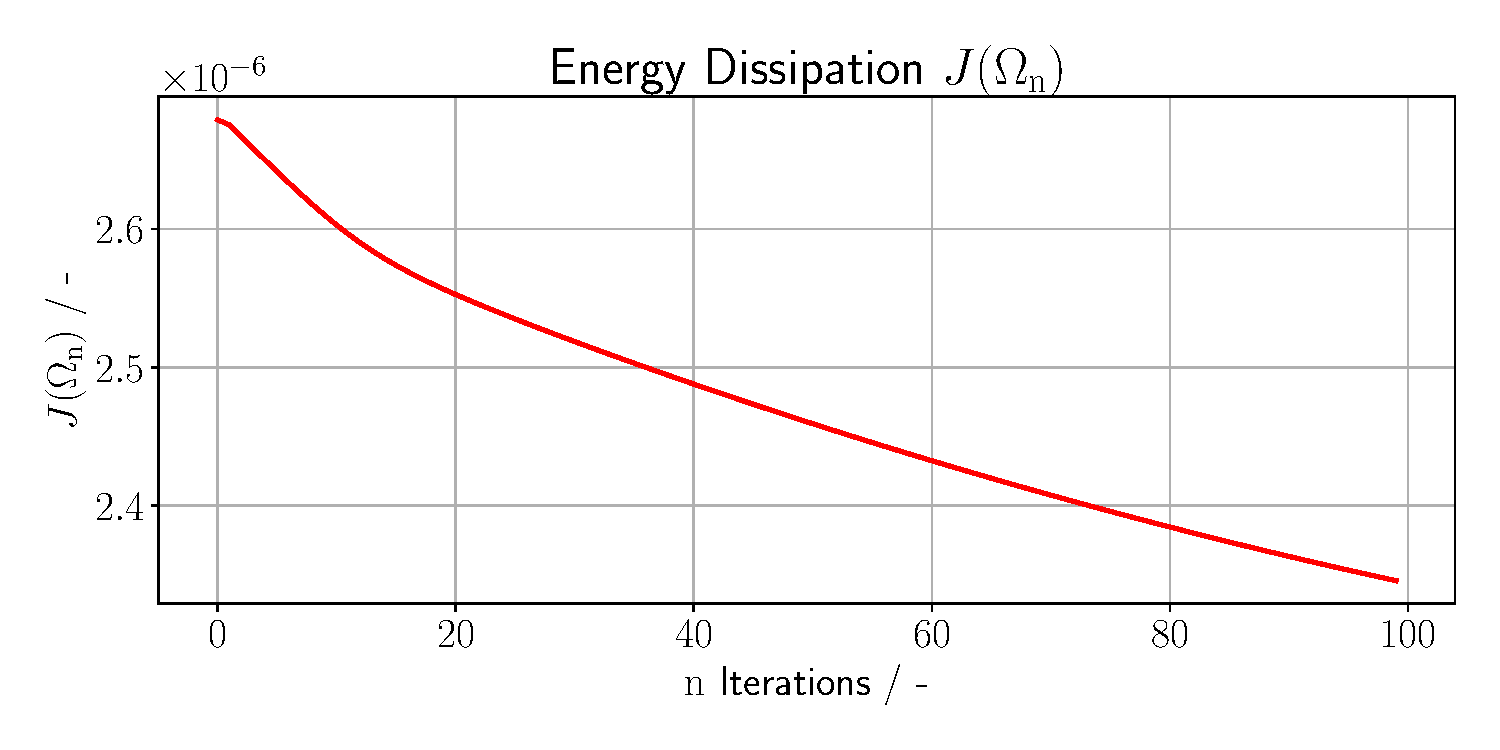
\includegraphics[width=1\textwidth]{figures/energy_diss_plot.pdf}
        \caption{Evaluation of Energy Dissipation on $\Omega$}
        \label{plot_ref_energy_diss}
    \end{center}
\end{figure}

In figure \ref{plot_ref_energy_diss}, convergence of the minimization problem can be observed. However, not
only convergence with respect tho the energy minimization is relevant in the posed problem. Since the 
Augmented Lagrangian (\ref{final_aug_lagrange}) also tracks the quantities $\mathrm{vol}(\Omega_{\mathrm{n}}), \,
\mathrm{\mathrm{bc}_x(\Omega_{\mathrm{n}})}, \, \mathrm{bc}_y(\Omega_{\mathrm{n}})$ by keeping them constant or rather penalize
deviations from the initial value, investigation of these values are also done subsequently.

\pagebreak
\begin{figure}
    \begin{center}
        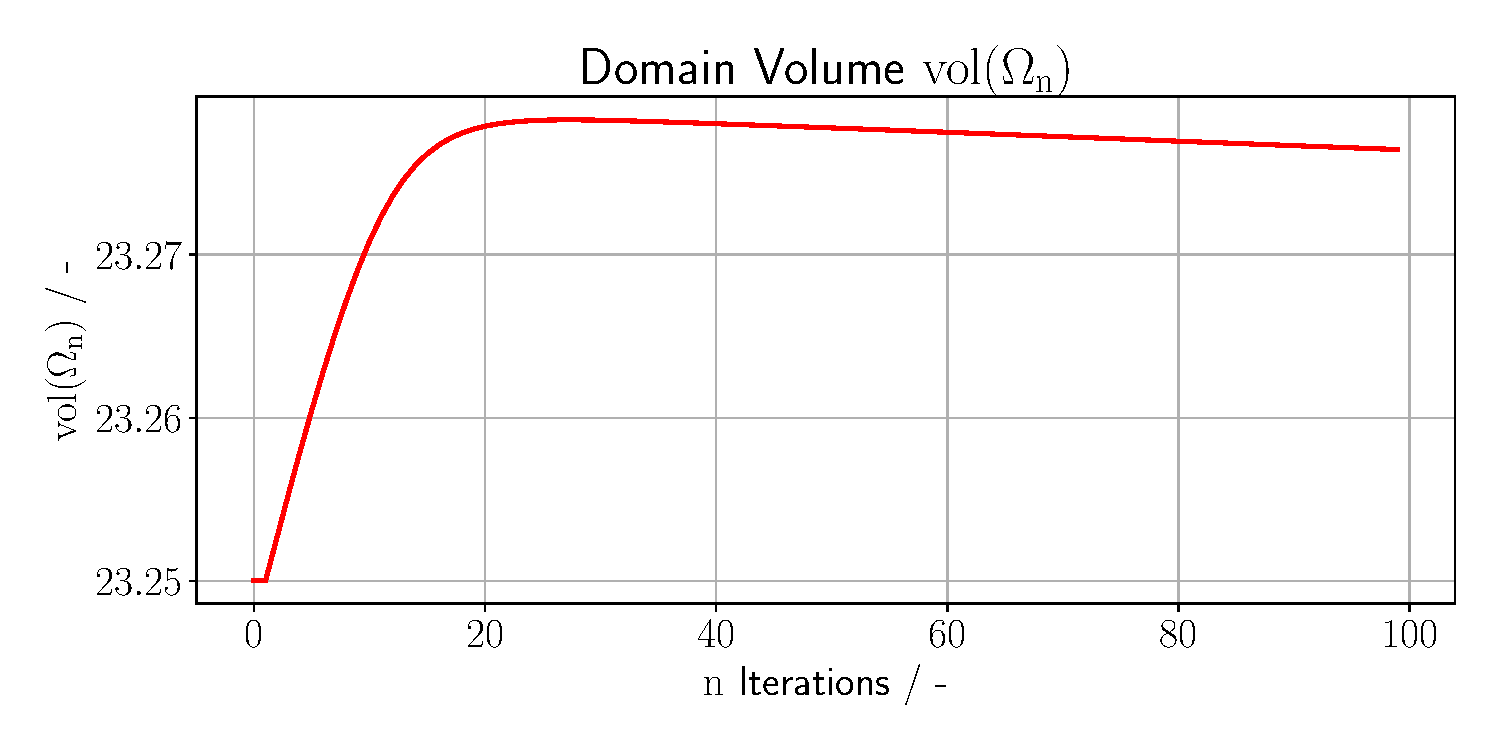
\includegraphics[width=0.8\textwidth]{figures/volume_plot.pdf}
        \caption{Volume of $\Omega$}
        \label{plot_ref_volume}
    \end{center}
\end{figure}
\begin{figure}
    \begin{minipage}{.5\textwidth}
        \centering
        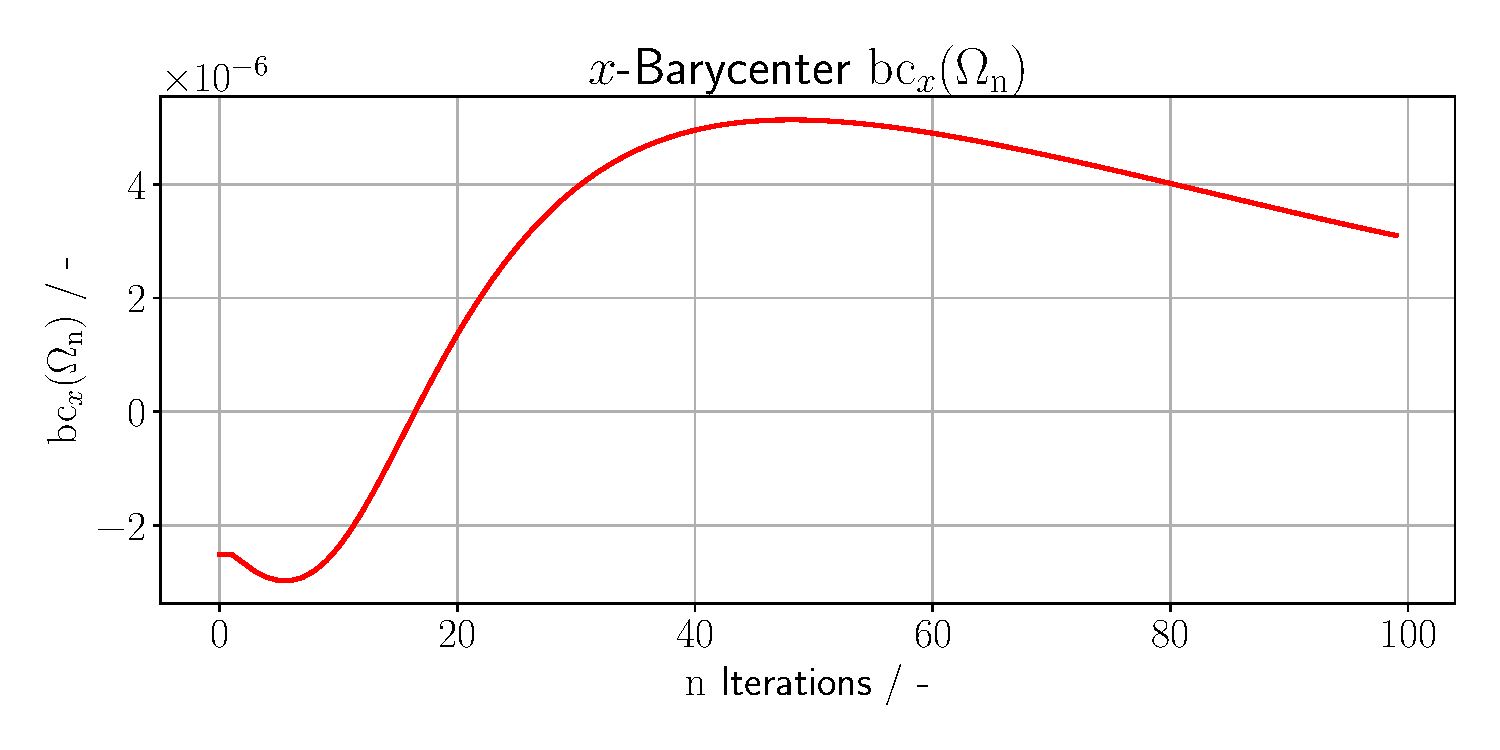
\includegraphics[width=1\textwidth]{figures/bc_x__plot.pdf}
        \caption{$x$ Component of Barycenter of $\Omega$}
        \label{plot_ref_bc_x}
    \end{minipage}
    \begin{minipage}{.5\textwidth}
        \centering
        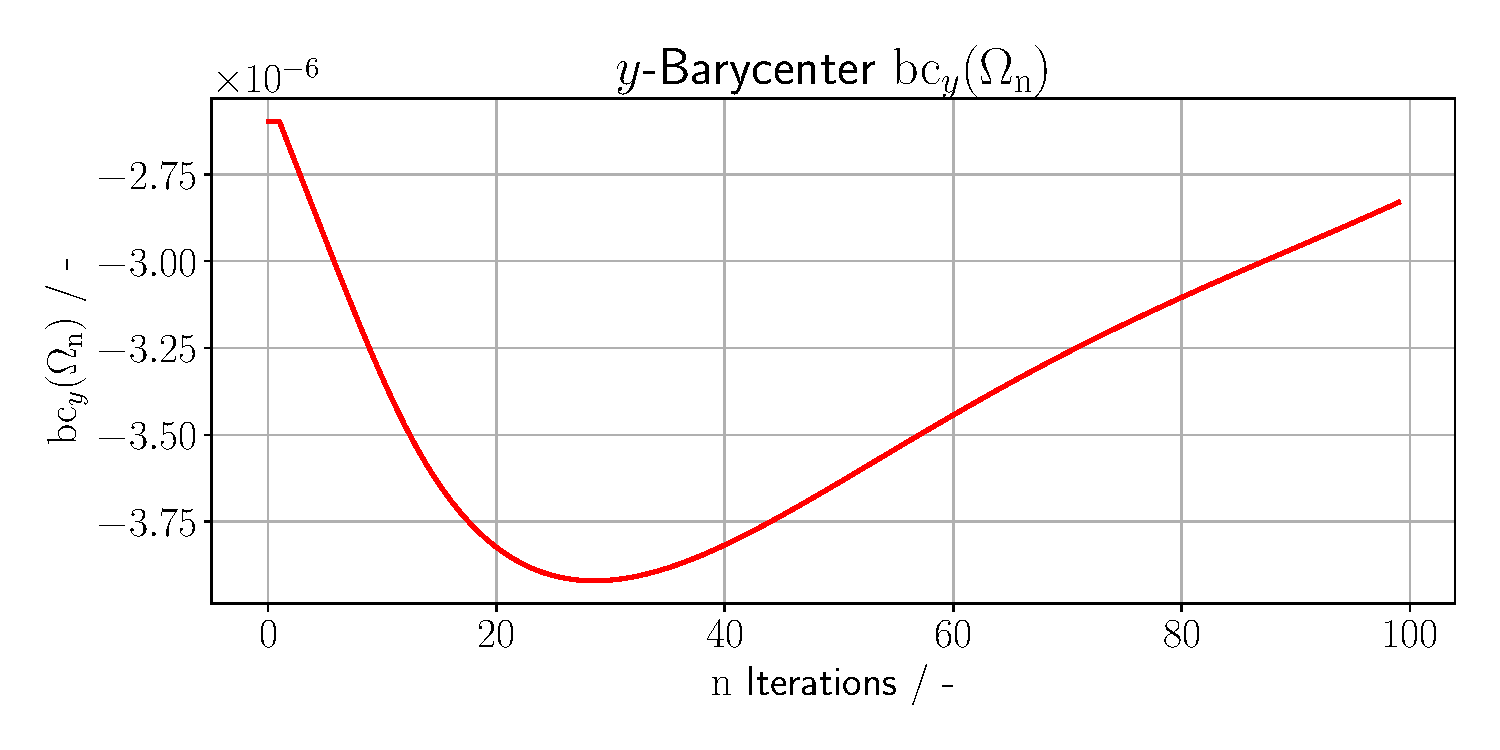
\includegraphics[width=1\textwidth]{figures/bc_y_plot.pdf}
        \caption{$y$ Component of Barycenter of $\Omega$}
        \label{plot_ref_bc_y}
    \end{minipage}
    \end{figure}

In figure \ref{plot_ref_volume}, oscillations around the initial value $\mathrm{vol}(\Omega_0)$ can be
be observed, which further underlines the approximative character of the Augmented Lagrangian Method
(\ref{final_aug_lagrange}). The same behaviour can be observed for the barycenters in $x$ and $y$
directions, which for a symmetric domain $\Omega$ with respects to the coordinate system should
both be 0.
\begin{figure}[h]
    \begin{minipage}{.5\textwidth}
        \centering
        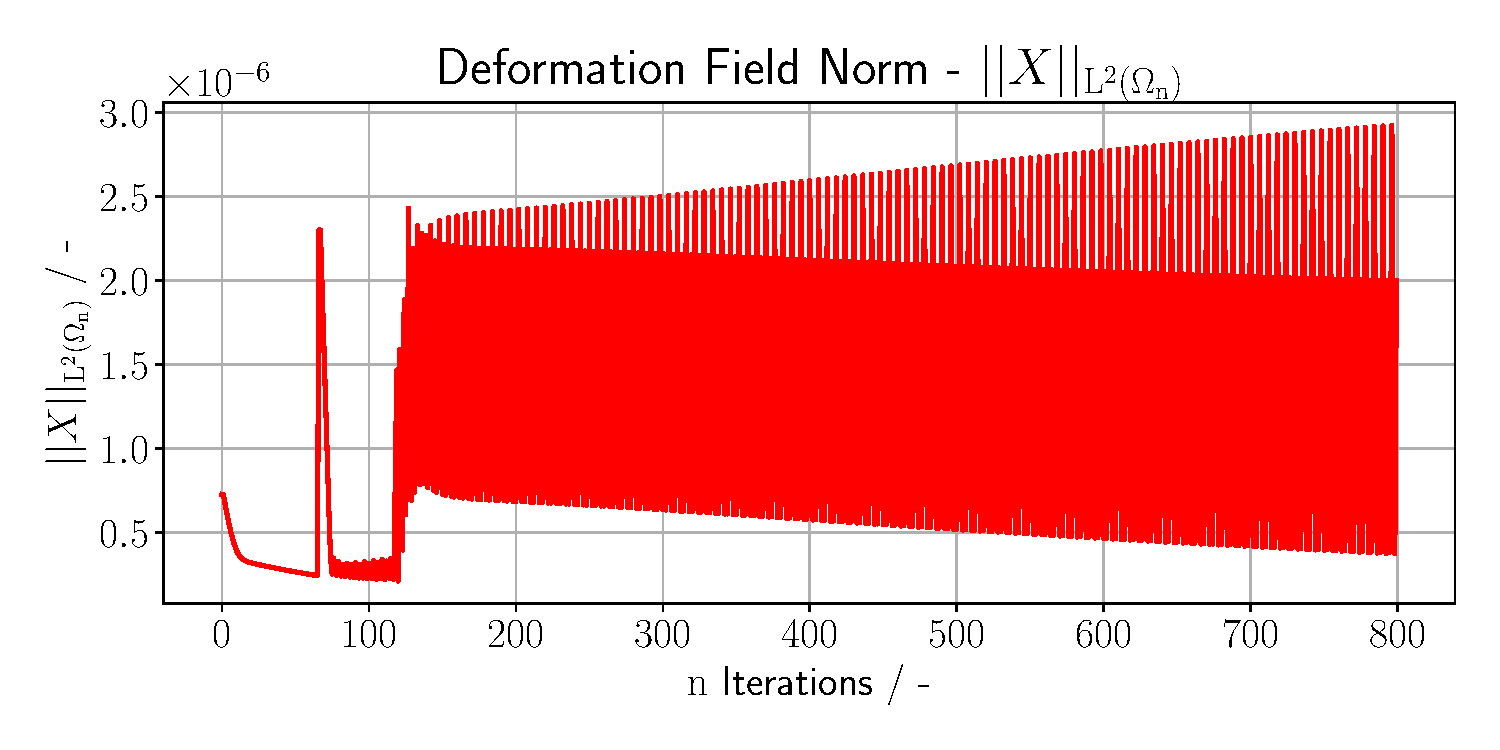
\includegraphics[width=1\textwidth]{figures/gfxnorm_plot.pdf}
        \caption{Norm of $X$ on Domain}
        \label{plot_ref_norm}
    \end{minipage}
    \begin{minipage}{.5\textwidth}
        \centering
        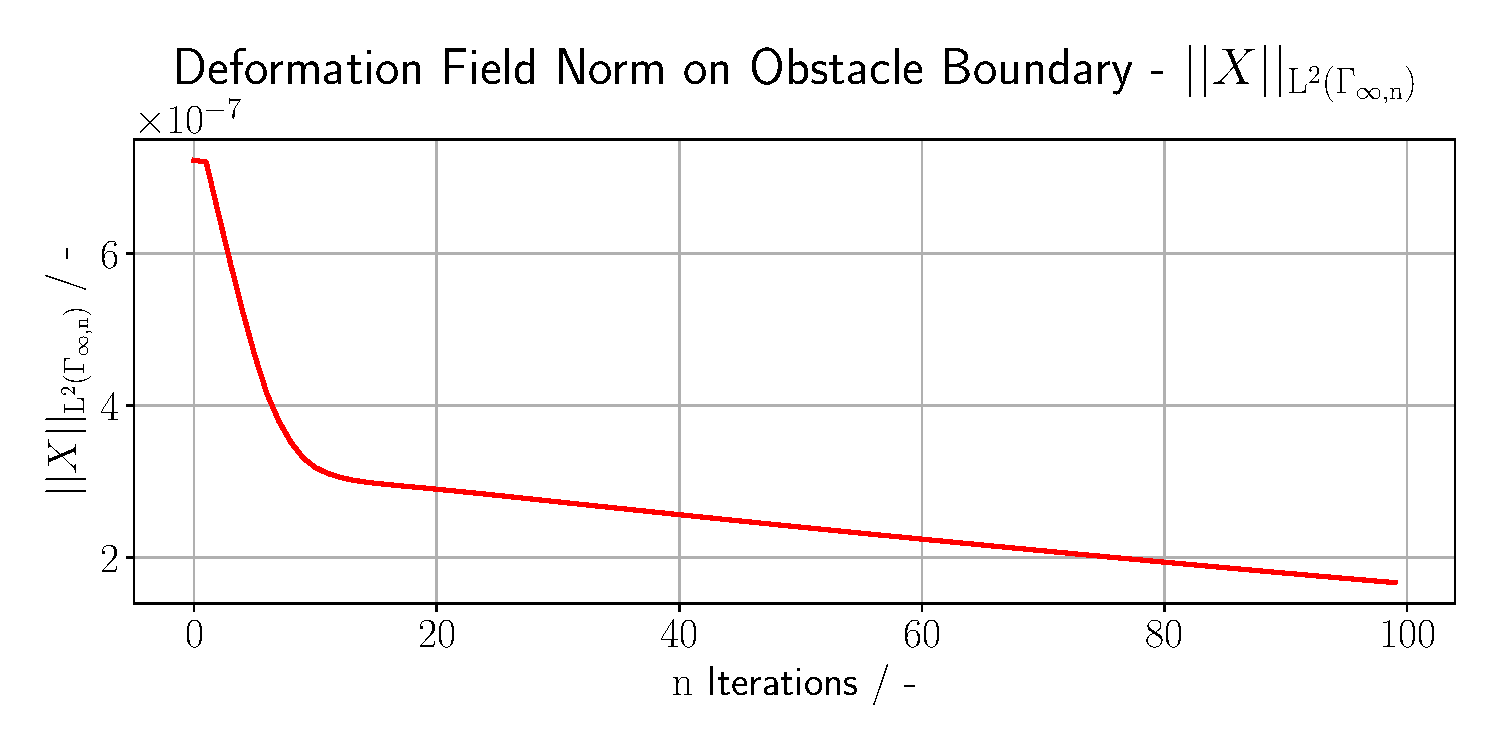
\includegraphics[width=1\textwidth]{figures/gfx_bndnorm_plot.pdf}
        \caption{Norm of $X$ on Boundary}
        \label{plot_ref_bndnorm}
    \end{minipage}
\end{figure}

In figures \ref{plot_ref_norm} and \ref{plot_ref_bndnorm} the $L^2$ norms on the domain
and the obstacle boundary are evaluated. These quantities have similar shape but a scaling factor of 2 
in between. In a subsequent Seminary Project, one could investigate their scaling impact for the iterations
further.

\pagebreak

\subsection{Cauchy-Riemann Constraint Impact on Mesh and Shape}

\begin{figure}[h]
    \begin{minipage}{.5\textwidth}
        \centering
        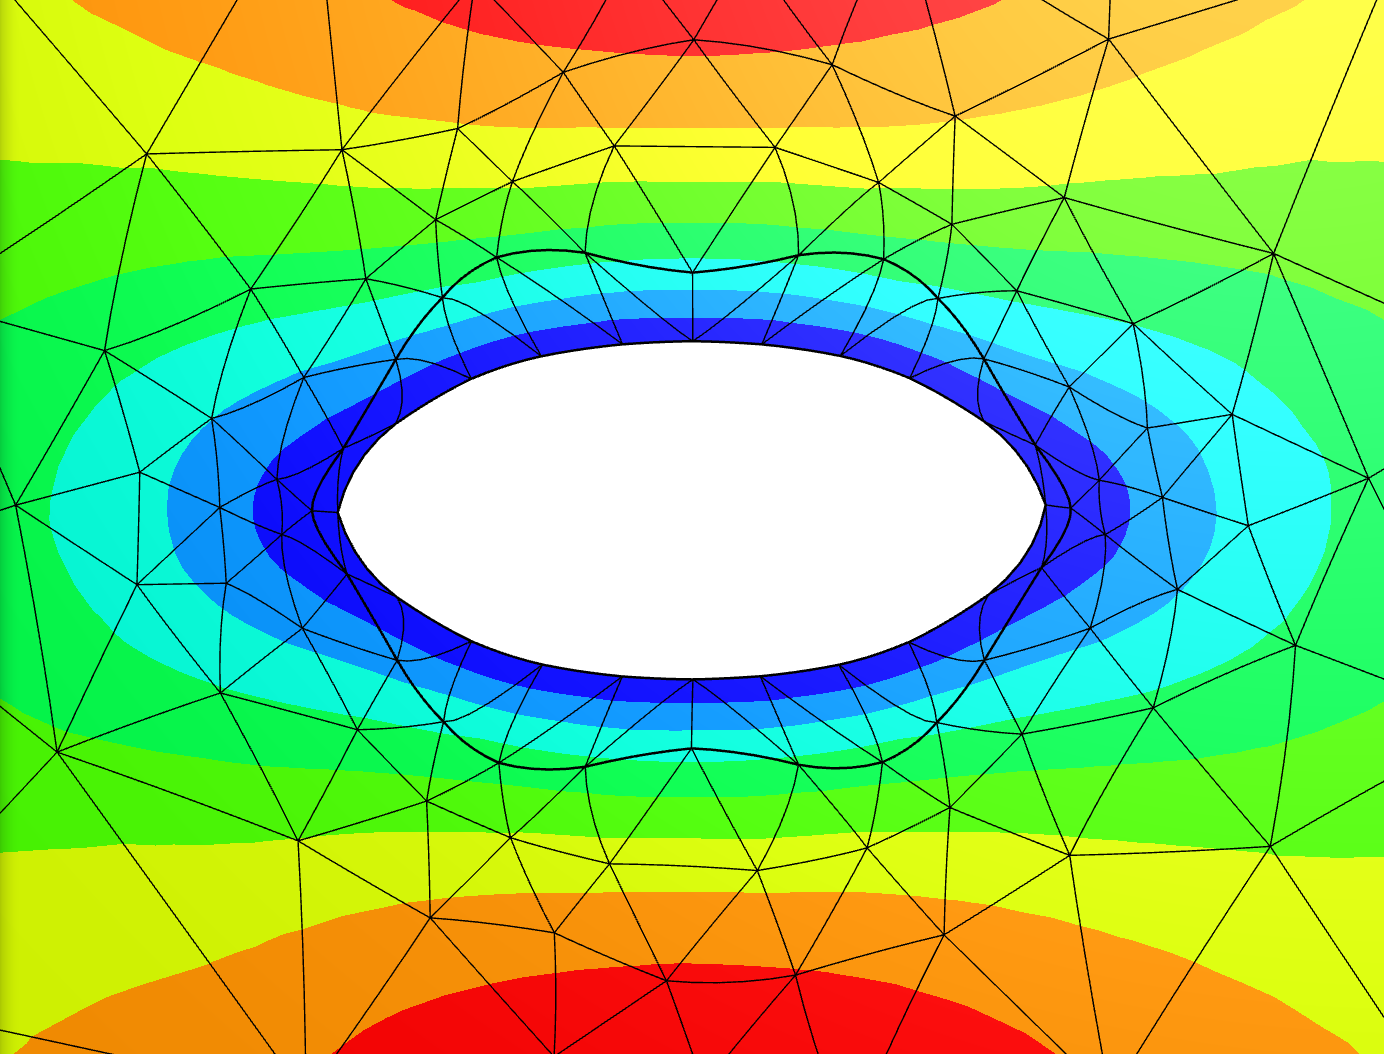
\includegraphics[width=0.97\textwidth]{figures/mesh_good.PNG}
        \caption{Final $\Omega$ with CR Constraint}
        \label{plot_ref_good_mesh_u}
    \end{minipage}
    \begin{minipage}{.5\textwidth}
        \centering
        
\includegraphics[width=1\textwidth]{figures/mesh_bad.PNG}
        \caption{Final $\Omega$ without CR Constraint}
        \label{plot_ref_bad_mesh_u}
    \end{minipage}
\end{figure}
\begin{figure}[h]
    \begin{minipage}{.5\textwidth}
        \centering
        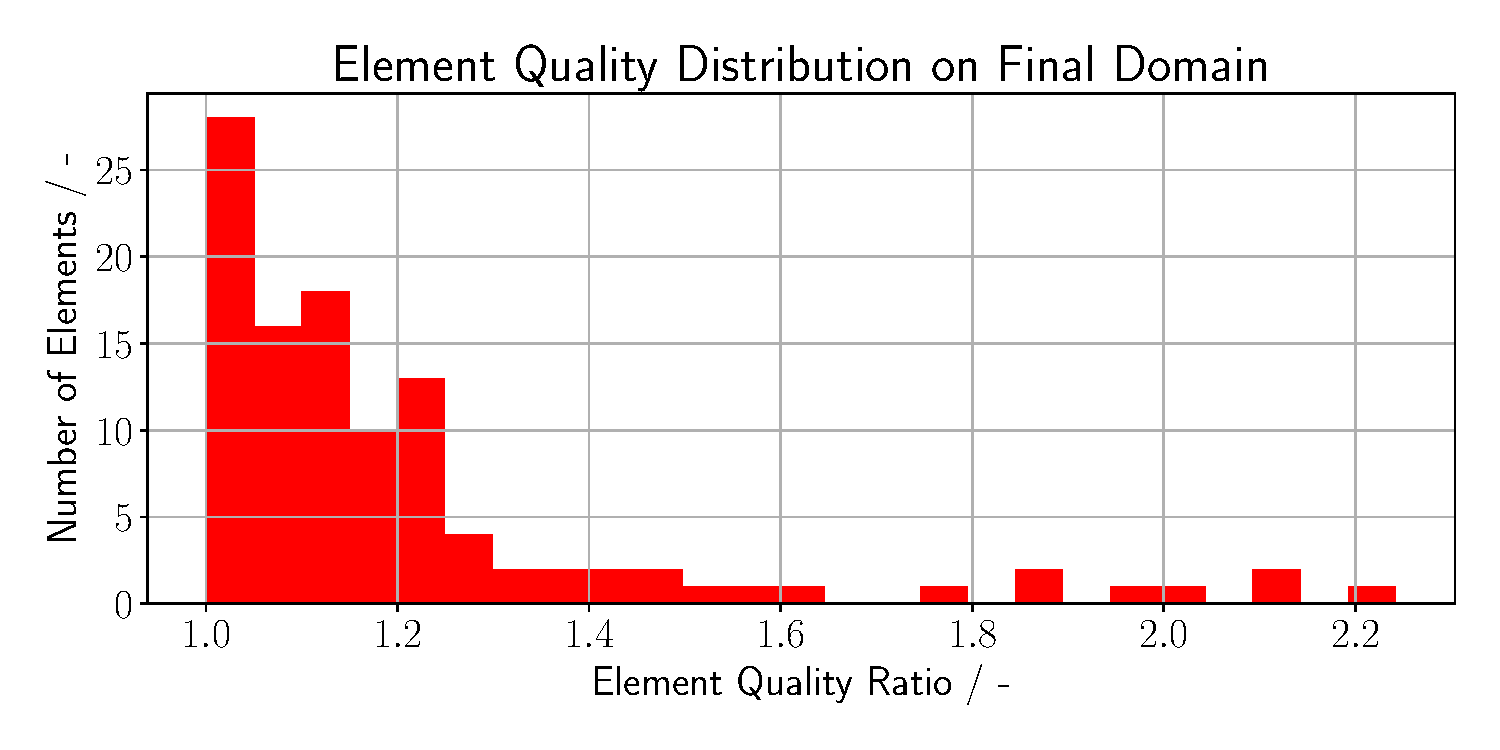
\includegraphics[width=1\textwidth]{figures/element_quality_hist.pdf}
        \caption{Element Quality with CR Constraint}
        \label{plot_ref_element_good}
    \end{minipage}
    \begin{minipage}{.5\textwidth}
        \centering
        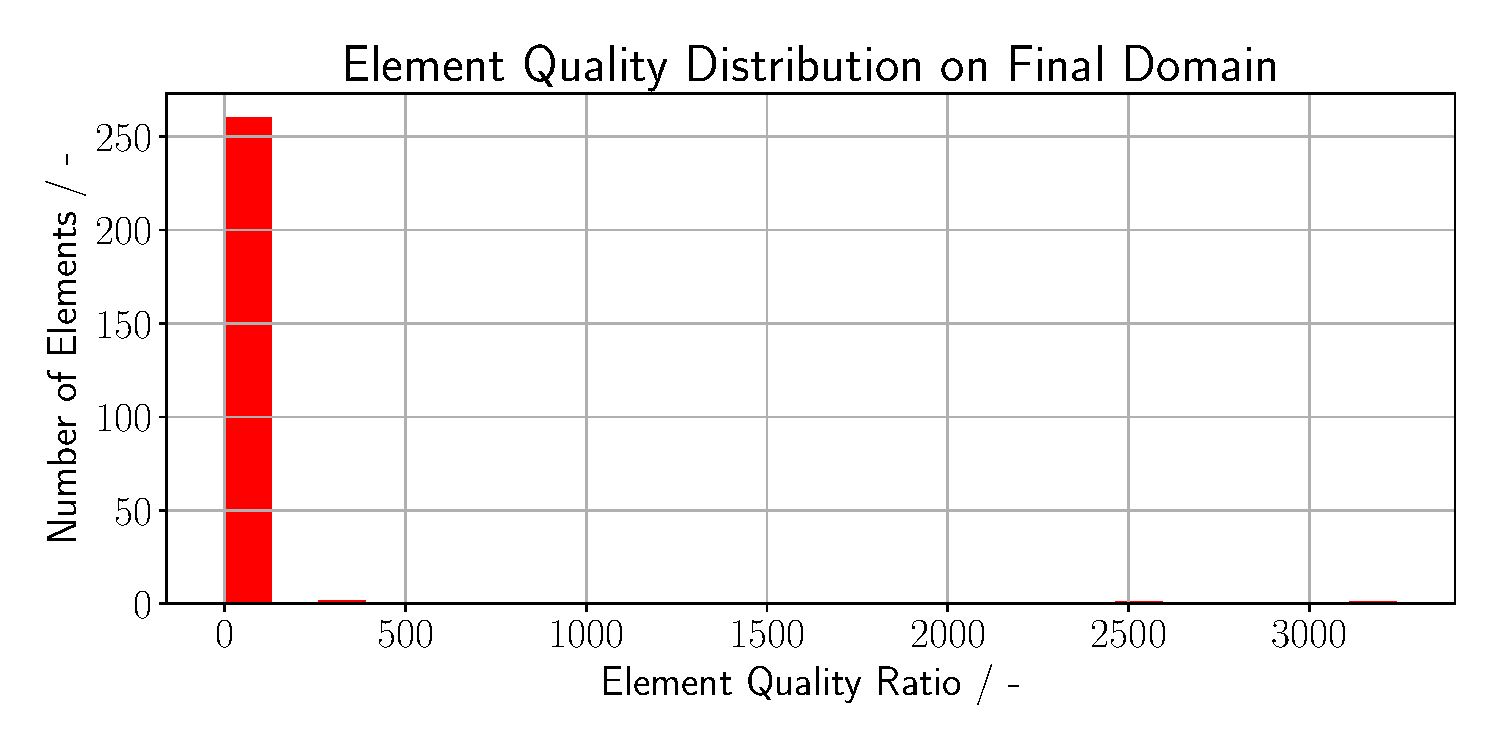
\includegraphics[width=1\textwidth]{figures/element_quality_hist_bad.pdf}
        \caption{Element Quality without CR Constraint}
        \label{plot_ref_element_bad}
    \end{minipage}
\end{figure}

In figures \ref{plot_ref_good_mesh_u} - \ref{plot_ref_element_bad}, the impact of the Cauchy-Riemann 
constraint can be observed. The mesh in figure \ref{plot_ref_bad_mesh_u} adjacent to the obstacle is
highly distorted and the solutions $(\mathbf{u},p)$ therefore not reliable anymore. The element quality 
at the tips is approximately 3000 without the CR constraint, as shown in figure \ref{plot_ref_element_bad}.
With applied CR constraint with $\alpha = 150$, the minimization after 800 iterations results in a acceptable
element quality distribution, as shown in figures \ref{plot_ref_good_mesh_u} and \ref{plot_ref_element_good}.

\pagebreak

\subsection{Cauchy-Riemann Constraint on Convergence Behaviour}
\begin{figure}[h]
    \begin{minipage}{.5\textwidth}
        \centering
        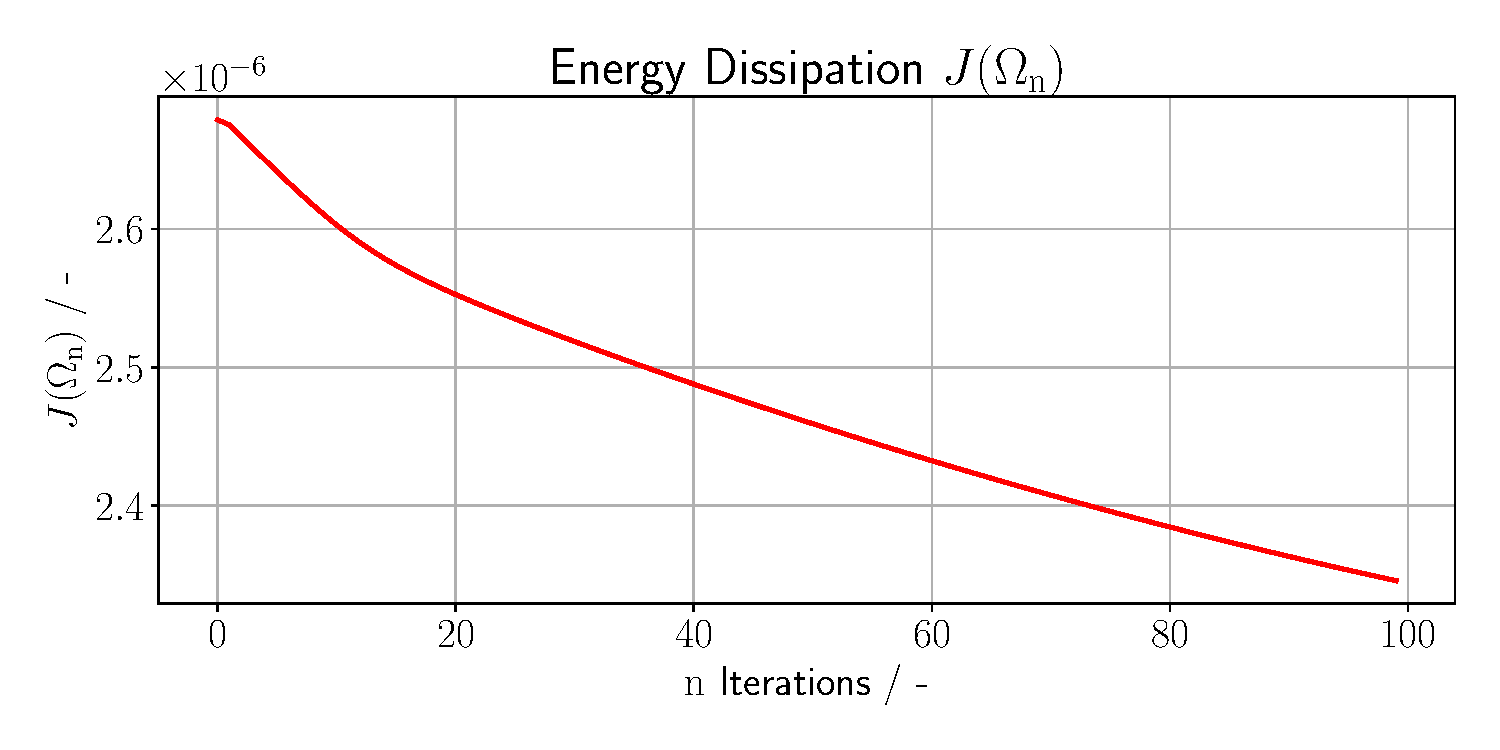
\includegraphics[width=1\textwidth]{figures/energy_diss_plot.pdf}
        \caption{Energy Diss. with CR Constraint}
        \label{plot_ref_energy_diss_good}
    \end{minipage}
    \begin{minipage}{.5\textwidth}
        \centering
        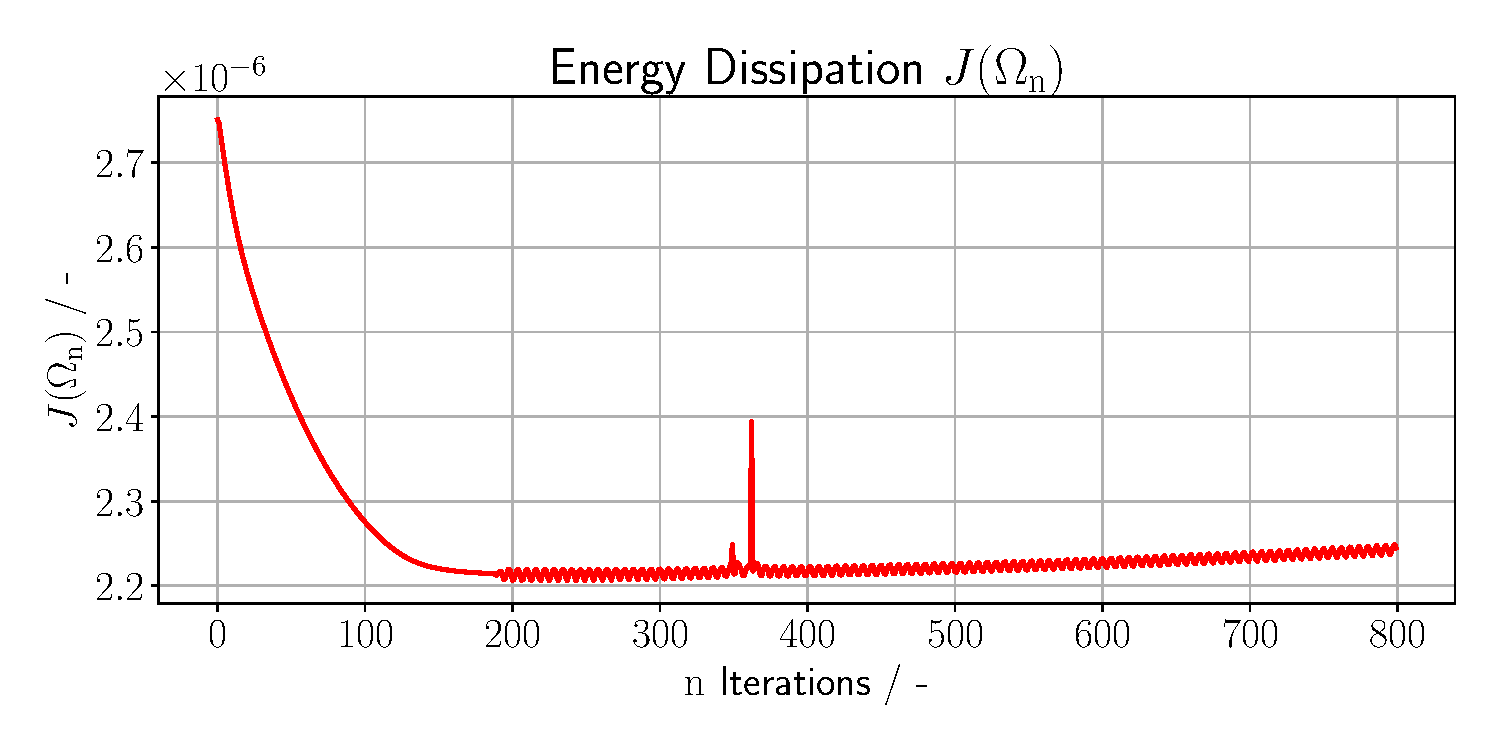
\includegraphics[width=1\textwidth]{figures/energy_diss_plot_bad.pdf}
        \caption{Energy Diss. without CR Constraint}
        \label{plot_ref_energy_diss_bad}
    \end{minipage}
\end{figure}
\begin{figure}[h]
    \begin{minipage}{.5\textwidth}
        \centering
        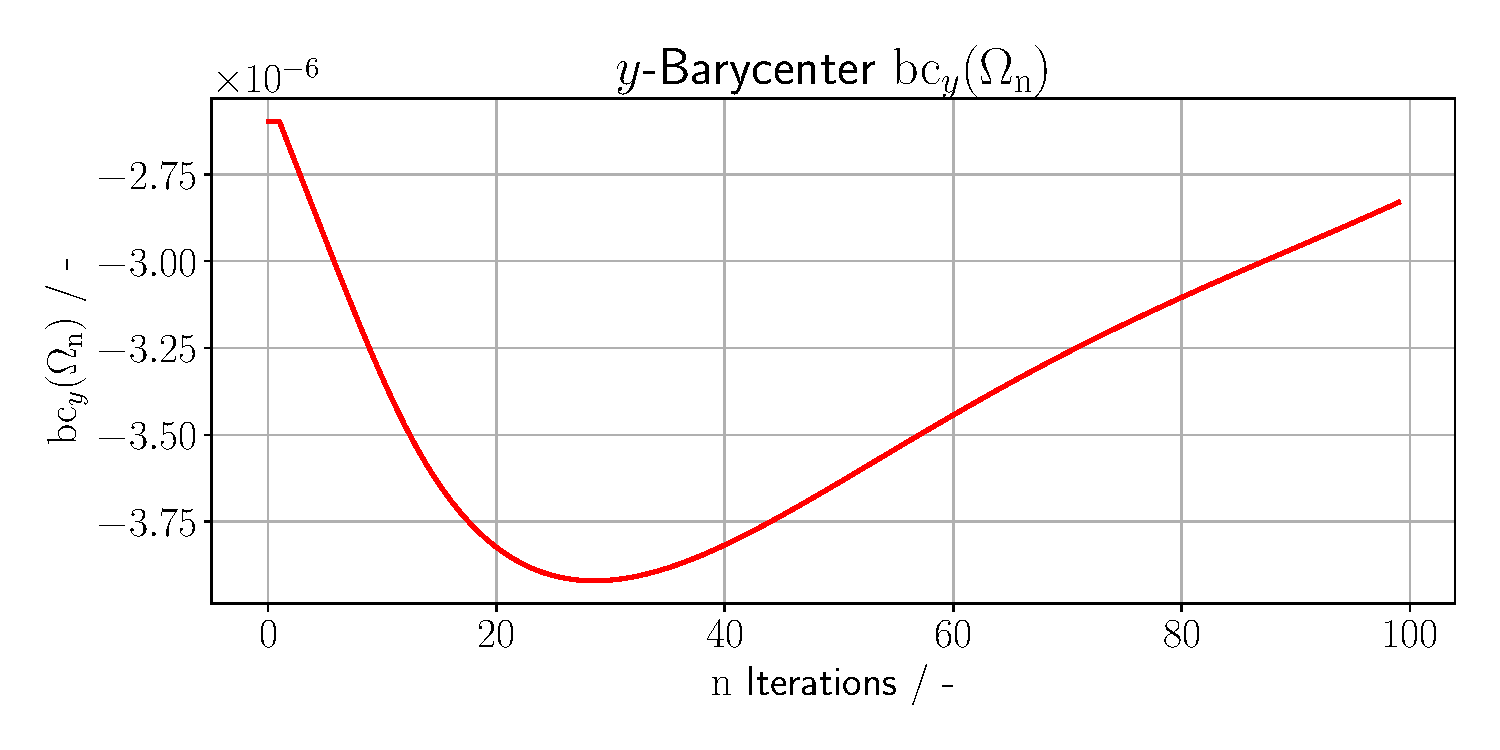
\includegraphics[width=1\textwidth]{figures/bc_y_plot.pdf}
        \caption{$y$-Barycenter with CR Constraint}
        \label{plot_ref_bc_y_good}
    \end{minipage}
    \begin{minipage}{.5\textwidth}
        \centering
        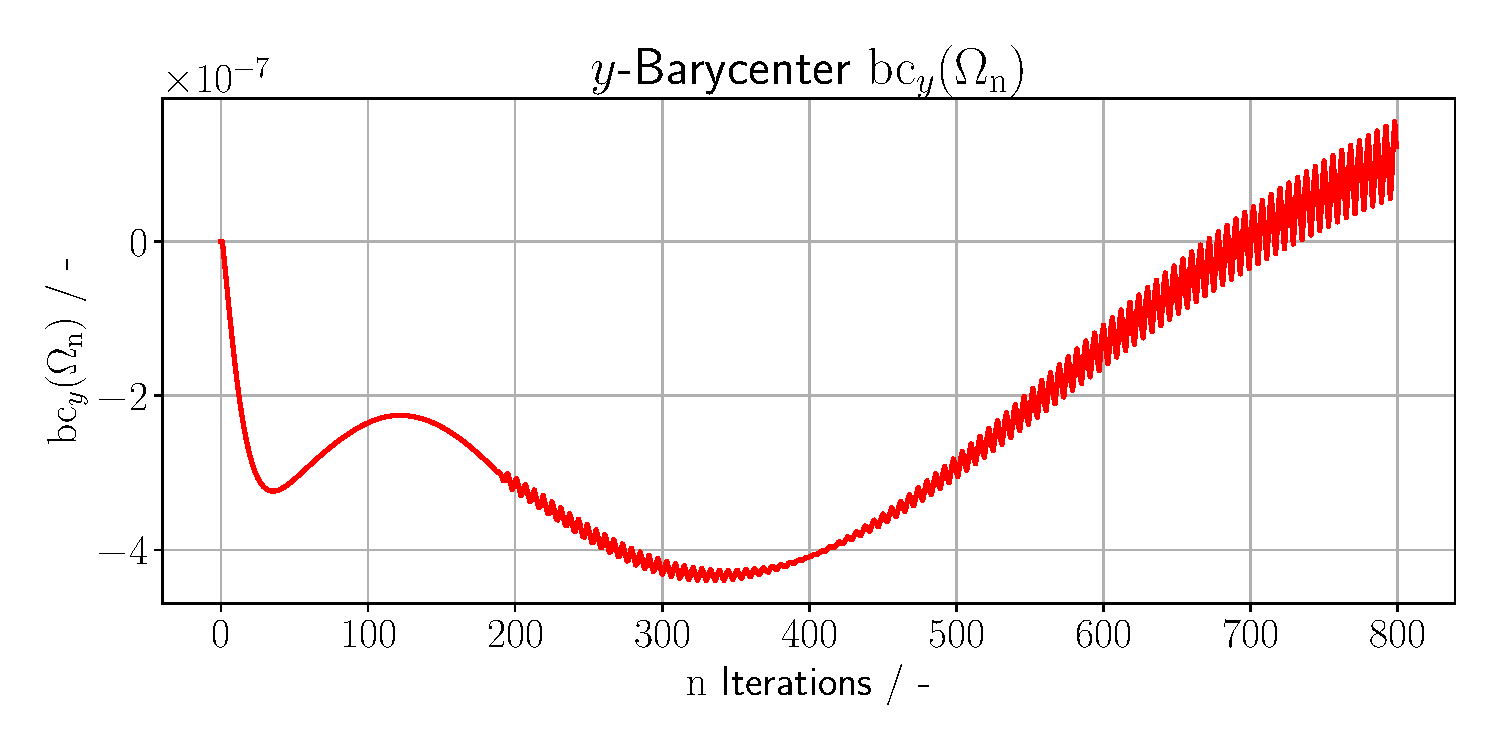
\includegraphics[width=1\textwidth]{figures/bc_y_plot_bad.pdf}
        \caption{$y$-Barycenter without CR Constraint}
        \label{plot_ref_bc_y_bad}
    \end{minipage}
\end{figure}
\begin{figure}[h]
    \begin{minipage}{.5\textwidth}
        \centering
        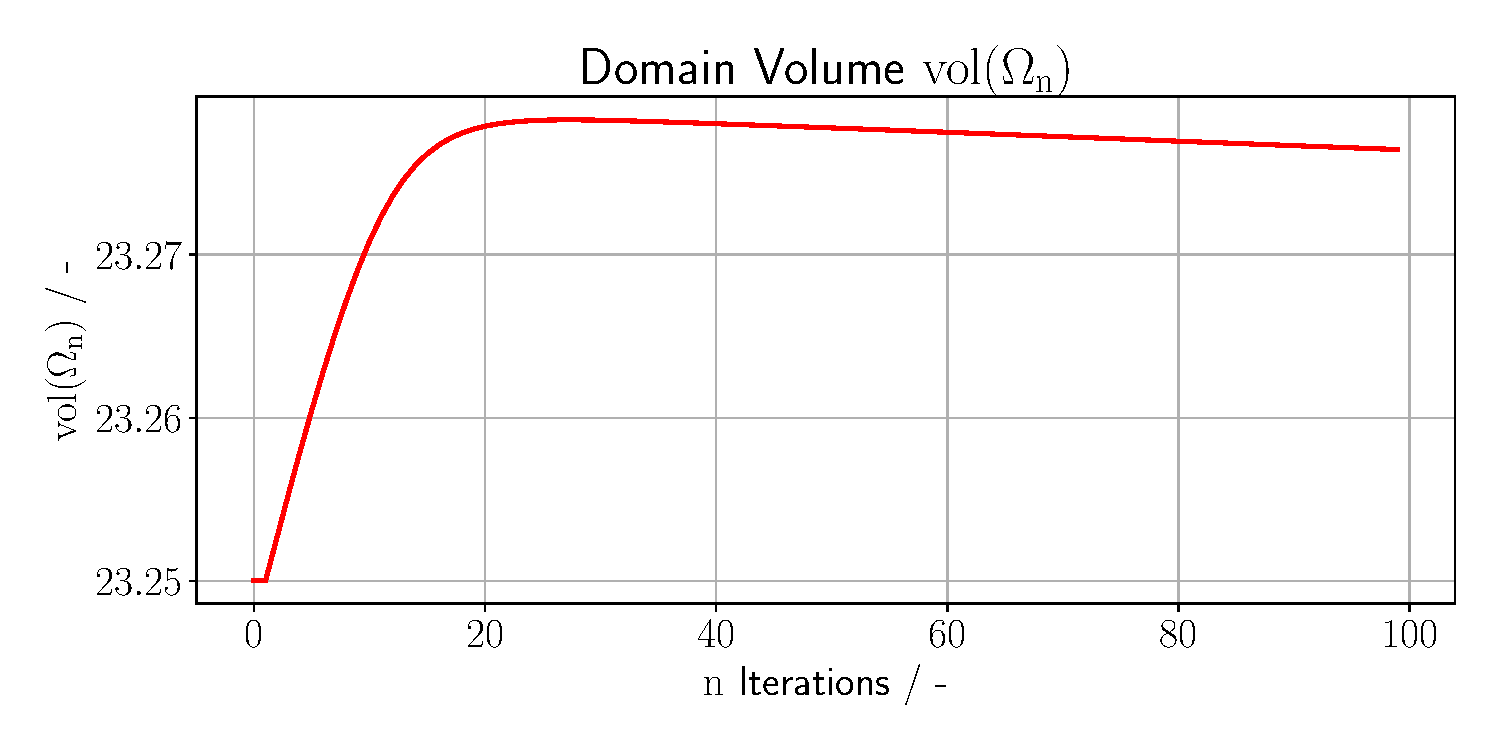
\includegraphics[width=1\textwidth]{figures/volume_plot.pdf}
        \caption{Volume with CR Constraint}
        \label{plot_ref_vol_good}
    \end{minipage}
    \begin{minipage}{.5\textwidth}
        \centering
        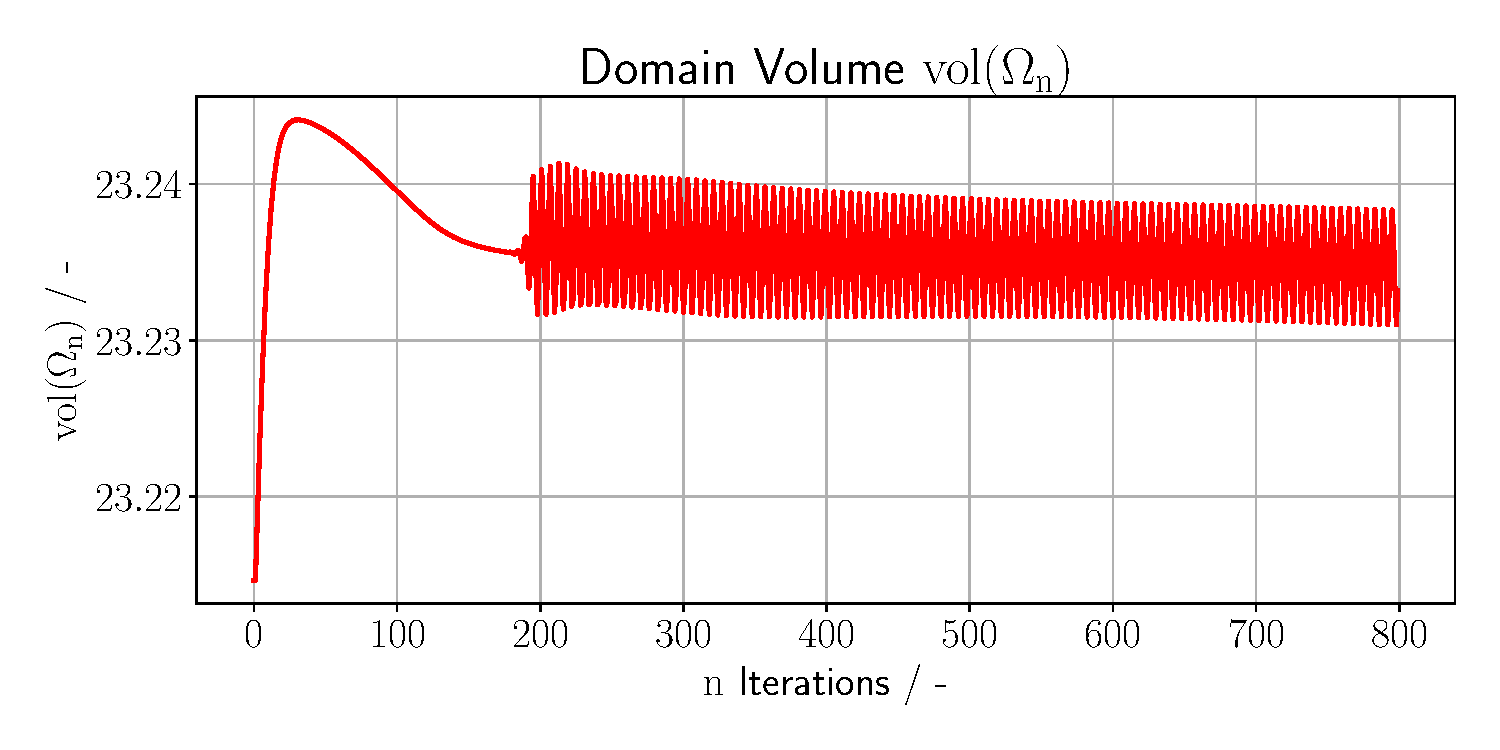
\includegraphics[width=1\textwidth]{figures/volume_plot_bad.pdf}
        \caption{Volume wihtout CR Constraint}
        \label{plot_ref_vol_bad}
    \end{minipage}
\end{figure}

In figure \ref{plot_ref_energy_diss_bad}, the energy dissipation increases again after 200 iterations,
while the $y$-barycenter in figure \ref{plot_ref_bc_y_bad} and the volume of $\Omega$ 
Figure \ref{plot_ref_vol_bad} are not nearly in the vicinity of the desired initial values.
For this PDE-Constrained Shape optimization setup, the CR-Equations are therefore even needed,
since no convergence can be observed without them for all tracked quantities.

\pagebreak

\pagebreak
%%%%%%%%%%%%%%%%%%%%%%%%%%%%%%%%%%%%%%%%%%%%%%%%%%%%%%%%%%%
%%%%%%%%%%%%%%%%%%%%%%%%%%%%%%%%%%%%%%%%%%%%%%%%%%%%%%%%%%%
%%%%%%%%%%%%%%%%%%%%%%%%%%%%%%%%%%%%%%%%%%%%%%%%%%%%%%%%%%%
%%%%%%%%%%%%%%%%%%%%%%%%%%%%%%%%%%%%%%%%%%%%%%%%%%%%%%%%%

%% During the document writing process, this single .tex file is used to let dasdyou write down a little to do list, just comment it out when the paper is done!

%%%%%%%%%%%%%%%%%%%%%%%%%%%%%%%%%%%%%%%%%%%%%%%%%%%%%%%%%%%
%%%%%%%%%%%%%%%%%%%%%%%%%%%%%%%%%%%%%%%%%%%%%%%%%%%%%%%%%%%
%%%%%%%%%%%%%%%%%%%%%%%%%%%%%%%%%%%%%%%%%%%%%%%%%%%%%%%%%%%
%%%%%%%%%%%%%%%%%%%%%%%%%%%%%%%%%%%%%%%%%%%%%%%%%%%%%%%%%

%%% Bibliography printing at this point! 
\printbibliography

%%% This is a hardcoded string to enforce it in the table of contents, if you want your "references" string in the TOC to be named differently, such as bibliography or so on, just change the third input to this command below to your desired references naming that should appear in the TOC
\addcontentsline{toc}{section}{References}


\pagebreak

%%%%%%%%%%%%%%%%%%%%%%%%%%%%%%%%%%%%%%%%%%%%%%%%%%%%%%%%%%%
%%%%%%%%%%%%%%%%%%%%%%%%%%%%%%%%%%%%%%%%%%%%%%%%%%%%%%%%%%%
%%%%%%%%%%%%%%%%%%%%%%%%%%%%%%%%%%%%%%%%%%%%%%%%%%%%%%%%%%%


%%% This is where the appendix .tex file is included, the settings to the appendix are changed in the settings.tex file
\begin{appendix}
\addappheadtotoc
\section{Python Code - PDE Constrained Shape Optimization in \fun{NGSolve}}
\label{app_a}


\begin{lstlisting}[language=Python, title=NGSolve Shape Optimization Code in Python, label=final_code]
from ngsolve import *
from netgen.geom2d import SplineGeometry
from ngsolve.webgui import Draw
import numpy as np
import matplotlib.pyplot as plt

geo = SplineGeometry()
h_coarse = 1
h_fine = 0.15
geo.AddRectangle( (-3,-2), (3, 2), bcs = ("top", "out", "bot", "in"), leftdomain=1, rightdomain=0, maxh=h_coarse) 
geo.AddCircle(c=(0, 0), r=0.6, leftdomain=2, rightdomain=1, bc="outer_cylinder", maxh=h_fine) 
geo.AddCircle(c=(0, 0), r=0.5, leftdomain=0, rightdomain=2, bc="cyl", maxh=h_fine) 
mesh = Mesh(geo.GenerateMesh(maxh=h_coarse))
mesh.Curve(2);
scene1 = Draw(mesh)

# Order of spaces for Taylor-Hood Elements
k = 2
V = H1(mesh,order=k, dirichlet="top|bot|cyl|in|out")
Q = H1(mesh,order=k-1)
FES = FESpace([V,V,Q])

ux,uy,p = FES.TrialFunction()
vx,vy,q = FES.TestFunction()

# stokes equation
def Equation(ux,uy,p,vx,vy,q):
    div_u = grad(ux)[0]+grad(uy)[1] # custom div
    div_v = grad(vx)[0]+grad(vy)[1]
    return (grad(ux)*grad(vx)+grad(uy)*grad(vy) + div_u*q + div_v*p)* dx

a = BilinearForm(FES)
a += Equation(ux,uy,p,vx,vy,q)
a.Assemble()

gfu = GridFunction(FES)
uinf = 0.0005
uin = CoefficientFunction((uinf))
gfu.components[0].Set(uin, definedon=mesh.Boundaries("in|top|bot|out"))

x_velocity = CoefficientFunction(gfu.components[0])
scene_state = Draw(x_velocity, mesh, "vel")

def solveStokes():
    res = gfu.vec.CreateVector()
    res.data = -a.mat * gfu.vec
    inv = a.mat.Inverse(FES.FreeDofs())
    gfu.vec.data += inv * res
    scene_state.Redraw()
solveStokes()

def calc_drag(gfu):
    ux = gfu.components[0]
    uy = gfu.components[1]
    return 0.5*(grad(ux)*grad(ux)+grad(uy)*grad(uy)).Compile()*dx

alpha = 1e-4
surf_t = CoefficientFunction(1)
surf_0 = Integrate(surf_t,mesh)

bc_tx = CoefficientFunction(x)
bc_ty = CoefficientFunction(y)
bc_0x = 1/surf_0*Integrate(bc_tx,mesh)
bc_0y = 1/surf_0*Integrate(bc_ty,mesh)

# Test and trial functions for shape derivate
VEC = H1(mesh, order=2, dim=2, dirichlet="top|bot|in|out")
PHI, X = VEC.TnT()
# gfset denotes the deformation of the original domain and will be updated during the shape optimization
gfset = GridFunction(VEC)
gfset.Set((0,0))
mesh.SetDeformation(gfset)
SetVisualization(deformation=True)

# deformation calculation
gfX = GridFunction(VEC)

ux = gfu.components[0]
uy = gfu.components[1]
p = gfu.components[2]

vol = Parameter(1)
vol.Set(Integrate(surf_t,mesh))

Lagrangian = Equation(ux,uy,p,ux,uy,p) + calc_drag(gfu)  

dJOmega = LinearForm(VEC)
# automatic shape differentiation
dJOmega += Lagrangian.DiffShape(X)

# volume side constraint
vol = Parameter(1)
vol.Set(Integrate(surf_t,mesh))
alpha0 = 1e-4
alpha = Parameter(alpha0)
dJOmega += 2*alpha*(vol-surf_0)*div(X)*dx

# barycenter x sideconstraint
beta0 = 1e-3
beta = Parameter(beta0)
bc_x = Parameter(1)
bc_x.Set((1/surf_0)*Integrate(bc_tx,mesh))
dJOmega += 2*beta*(bc_x-bc_0x)*((1/vol**2)*div(X)*x+(1/vol)*div(X)*x*sum(gfset.vecs[0].data)[0])*dx

# barycenter y sideconstraint
bc_y = Parameter(1)
bc_y.Set((1/surf_0)*Integrate(bc_ty,mesh))
dJOmega += 2*beta*(bc_y-bc_0y)*((1/vol**2)*div(X)*y+(1/vol)*div(X)*y*sum(gfset.vecs[0].data)[1])*dx

b = BilinearForm(VEC)
b += (InnerProduct(grad(X),grad(PHI)+grad(PHI).trans)).Compile() *dx + (InnerProduct(X,PHI)).Compile()*dx

#Cauchy-Riemann Penalisation
gamma0 = 25
gamma = Parameter(gamma0)
zeta = 150
b += zeta*(PHI.Deriv()[0,0] - PHI.Deriv()[1,1])*(X.Deriv()[0,0] - X.Deriv()[1,1])*dx
b += zeta*(PHI.Deriv()[1,0] - PHI.Deriv()[0,1])*(X.Deriv()[1,0] - X.Deriv()[0,1])*dx

def updateParams(v=False):
    vol.Set(Integrate(surf_t,mesh))
    bc_x.Set((1/surf_0)*Integrate(bc_tx,mesh))
    bc_y.Set((1/surf_0)*Integrate(bc_ty,mesh))
    if(v):
        print(vol.Get(), bc_x.Get(), bc_y.Get())
updateParams()

def increaseParams(k=2,v=False):
    alpha.Set(alpha.Get()*k)
    beta.Set(beta.Get()*k)
    gamma.Set(gamma.Get()*k)
    if(v):
        print("alpha: ", alpha.Get(), ", beta: ", beta.Get(), ", gamma: ", gamma.Get())

        def SolveDeformationEquation():
        rhs = gfX.vec.CreateVector()
        rhs.data = dJOmega.vec - b.mat * gfX.vec
        update = gfX.vec.CreateVector()
        update.data = b.mat.Inverse(VEC.FreeDofs()) * rhs
        gfX.vec.data += update

gfset.Set((0,0))
mesh.SetDeformation(gfset)
scene.Redraw()

updateParams()
alpha0 = 1e-4
beta0 = 1e-0
gamma0 = 1e2
alpha.Set(alpha0)
beta.Set(beta0)
gamma.Set(gamma0)

a.Assemble()
solveStokes()

data = [[] for x in range(7)]

iter_max = 800

# try parts of loop
mesh.SetDeformation(gfset)
scene.Redraw()

c = 0

# input("Press enter to start optimization")
for i in range(0,iter_max):
    mesh.SetDeformation(gfset)
    scene.Redraw()
    scene_state.Redraw()
    
    if i%50 == 0:
        print('drag at iteration', i, ': ', Integrate(calc_drag(gfu), mesh))
        
    titles = ["Energy Dissipation","Volume","bc_x","bc_y","scale","gfxnorm","gfxbndnorm"] # collecting data
    data[0].append(Integrate(calc_drag(gfu),mesh))
    data[1].append(vol.Get())
    data[2].append(bc_x.Get())
    data[3].append(bc_y.Get())
    
    a.Assemble()
    solveStokes()
    
    b.Assemble()
    dJOmega.Assemble()
    SolveDeformationEquation()
    updateParams()
    
    mesh.UnsetDeformation()
    
    gfxnorm = Norm(gfX.vec)
    gfxbndnorm = Integrate(sqrt(gfX**2),mesh,BND)
    data[6].append(gfxbndnorm)
    #scale = 0.1 / Norm(gfX.vec)
    scale = 0.01 / gfxnorm
    data[4].append(scale)
    data[5].append(gfxnorm)
    
    
    c += 1
    #if(gfxnorm < 1e-5):
    if(gfxbndnorm < 1e-7 and c > 50):
        if alpha.Get() < 100:
            increaseParams(5,True)
            c = 0
        else:
            print("alpha too big")
            break
            
    gfset.vec.data -= scale * gfX.vec
\end{lstlisting}

\vfill

\end{appendix}


%%%%%%%%%%%%%%%%%%%%%%%%%%%%%%%%%%%%%%%%%%%%%%%%%%%%%%%%%%%
%%%%%%%%%%%%%%%%%%%%%%%%%%%%%%%%%%%%%%%%%%%%%%%%%%%%%%%%%%%
%%%%%%%%%%%%%%%%%%%%%%%%%%%%%%%%%%%%%%%%%%%%%%%%%%%%%%%%%%%


\end{document}

